\documentclass[12pt,a4paper]{article}

\usepackage[margin=1in]{geometry}
\usepackage{graphicx}
\usepackage{hyperref}
\usepackage{amsmath}
\usepackage{amsfonts}
\usepackage{booktabs}
\usepackage{setspace}
\usepackage{array}
\usepackage{caption}
\usepackage{subcaption}
\usepackage{float}
\usepackage{xcolor}
\usepackage{listings}
\usepackage{color}

\definecolor{codegreen}{rgb}{0,0.6,0}
\definecolor{codegray}{rgb}{0.5,0.5,0.5}
\definecolor{codepurple}{rgb}{0.58,0,0.82}
\definecolor{backcolour}{rgb}{0.95,0.95,0.92}

\lstdefinestyle{mystyle}{
    backgroundcolor=\color{backcolour},   
    commentstyle=\color{codegreen},
    keywordstyle=\color{magenta},
    numberstyle=\tiny\color{codegray},
    stringstyle=\color{codepurple},
    basicstyle=\ttfamily\footnotesize,
    breakatwhitespace=false,         
    breaklines=true,                 
    captionpos=b,                    
    keepspaces=true,                 
    numbers=left,                    
    numbersep=5pt,                  
    showspaces=false,                
    showstringspaces=false,
    showtabs=false,                  
    tabsize=2
}

\lstset{style=mystyle}

\onehalfspacing

\title{\textbf{EN639: Forecasting of Offshore Wind Power}}

\author{
\textbf{Rahul Kumar (23B1212)}
}

\date{}

\begin{document}

\maketitle

\section*{Objective}

\begin{itemize}
\item Review offshore wind power forecasting methodologies from international and Indian perspectives.
\item Evaluate advantages, limitations, and applicability of different forecasting approaches.
\item Develop an effective wind power forecasting model using an appropriate programming platform.
\item Validate forecasting accuracy using real wind generation data from a Renewable Energy (RE)-rich site.
\end{itemize}

\section*{Major Deliverables}

\begin{enumerate}
\item Literature review on wind power forecasting.
\item Comparative assessment of forecasting techniques.
\item Forecasting model implementation.
\item Validation results using actual generation data.
\item Final project report.
\end{enumerate}

\newpage

\section{Introduction}

\begin{figure}[H]
\centering
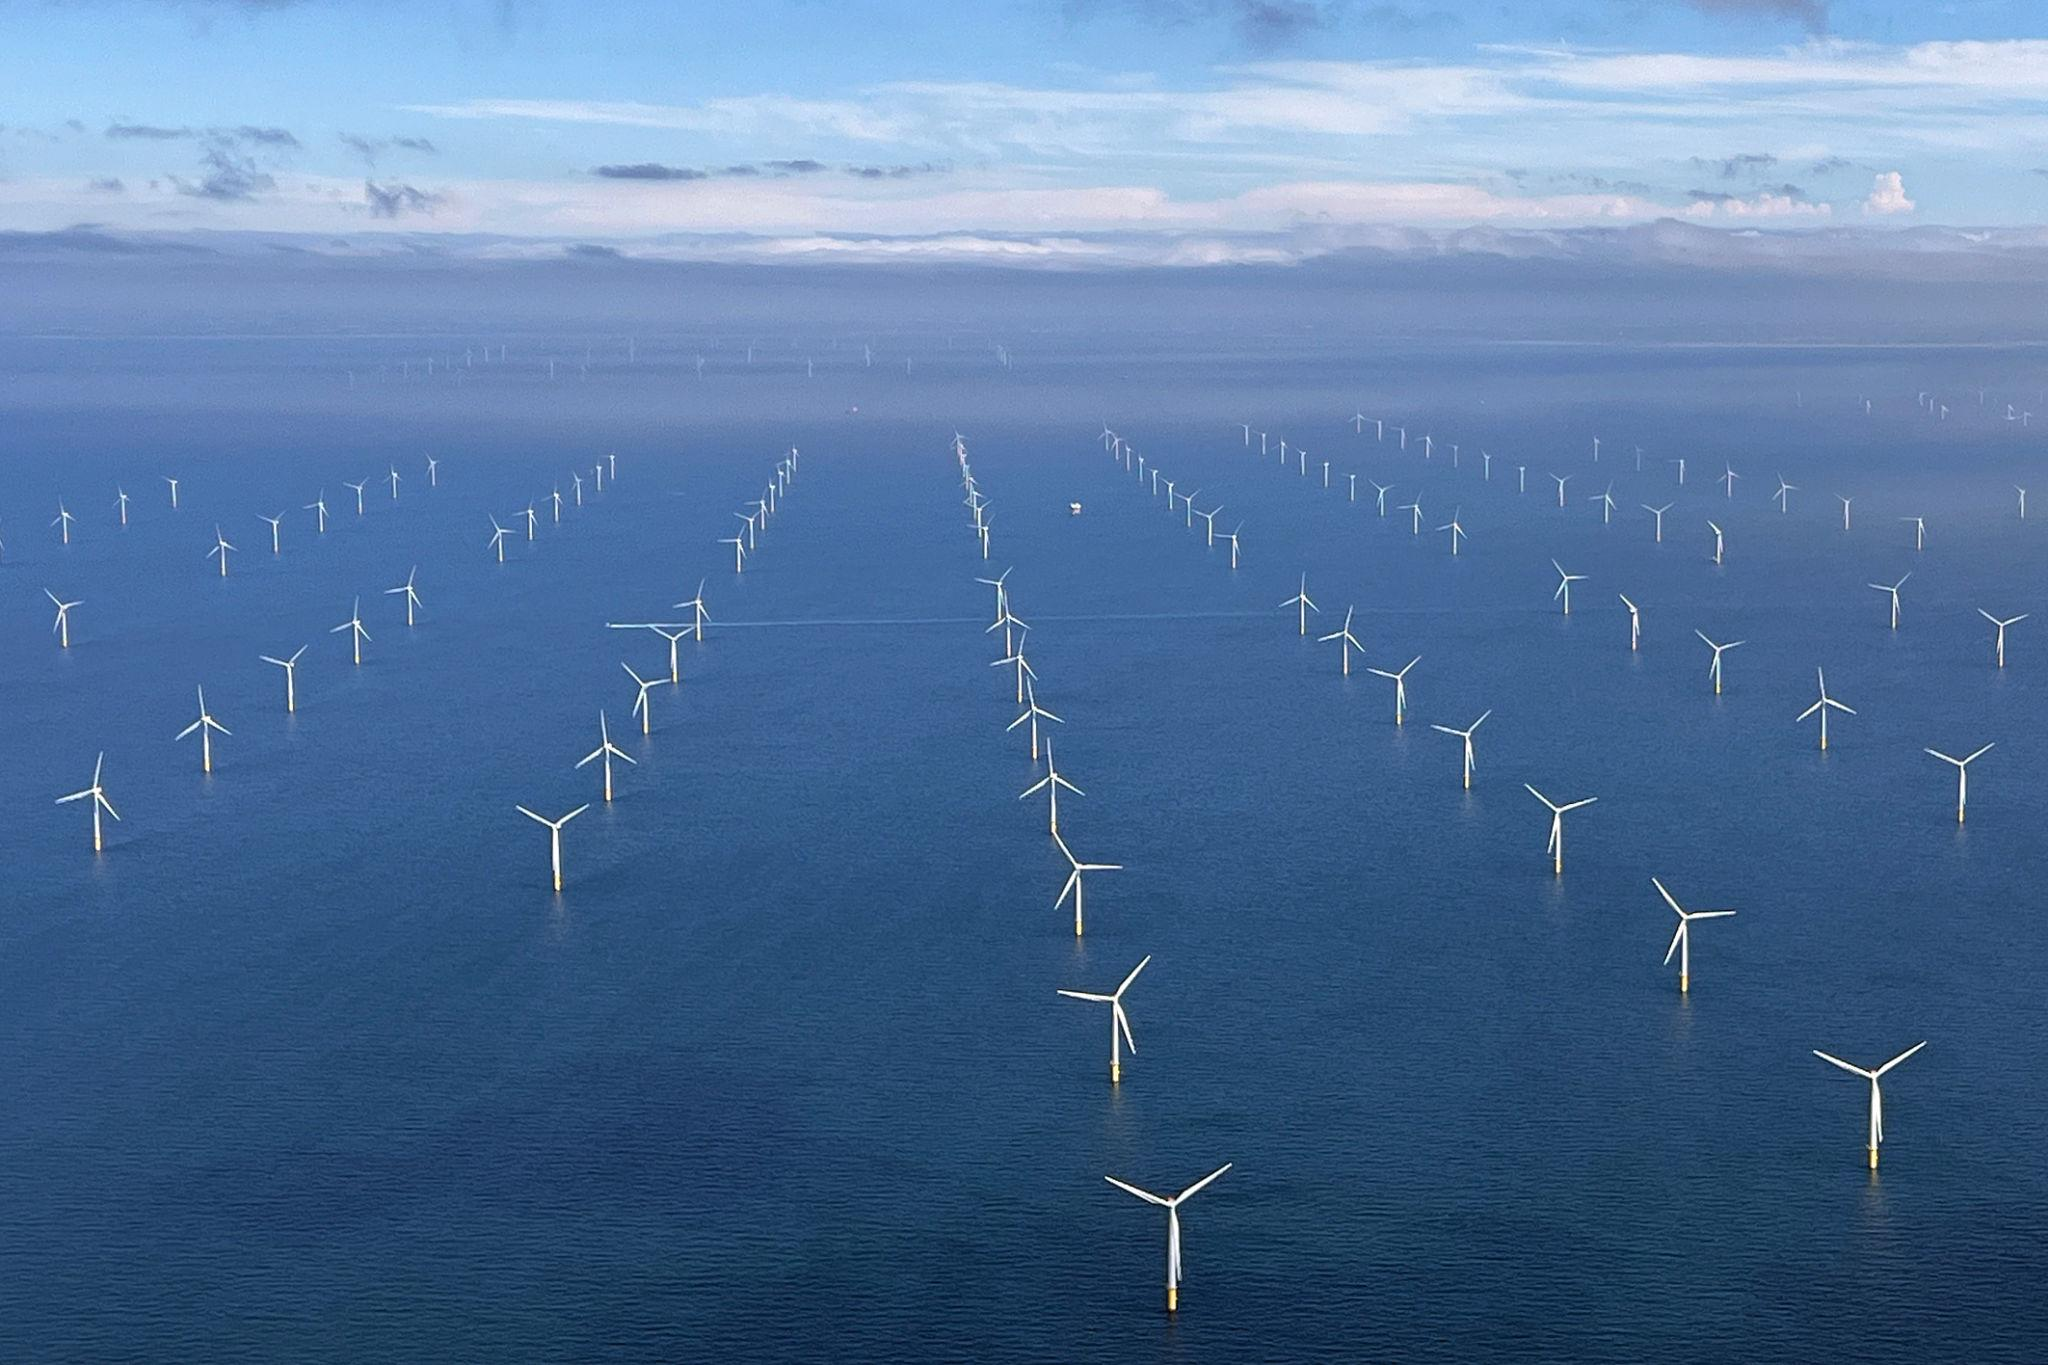
\includegraphics[width=1\textwidth]{c.jpg}
\caption{Typical offshore wind farm used for large-scale renewable electricity generation}
\label{fig:offshore_farm}
\end{figure}

Offshore wind energy has emerged as an important source of renewable electricity across the world. Wind speeds over oceans are generally stronger and more consistent than those over land because ocean surfaces have low surface roughness and reduced obstacles. As a result, offshore wind farms can produce larger and more stable amounts of power compared to many onshore wind installations.

\subsection{Wind Speed and Power Generation}

The electrical power produced by a wind turbine is strongly dependent on wind speed. A simplified physical relationship between wind speed and power output can be expressed as:

\begin{equation}
P = \frac{1}{2} \rho A v^3 C_p
\label{eq:power}
\end{equation}

where

\begin{itemize}
\item $P$ = power produced by the turbine (Watts)
\item $\rho$ = air density (kg/m³)
\item $A$ = rotor swept area of the turbine blades (m²)
\item $v$ = wind speed (m/s)
\item $C_p$ = power coefficient representing turbine efficiency (maximum theoretical value is 0.593, known as the Betz limit)
\end{itemize}

Equation \ref{eq:power} shows that power output is proportional to the cube of wind speed. Therefore, even small variations in wind speed can lead to large changes in power generation. This strong nonlinear relationship is one of the main reasons why accurate wind forecasting is essential for reliable power system operation.

\section{Forecasting Horizons in Offshore Wind Prediction}

Wind power forecasting is usually classified according to the prediction time horizon. Different forecasting horizons support different operational decisions in power system.

\begin{table}[H]
\centering
\caption{Classification of Wind Power Forecasting Horizons}
\label{tab:horizons}
\begin{tabular}{|p{3.5cm}|p{3.5cm}|p{8cm}|}
\hline
\textbf{Category} & \textbf{Forecast Horizon} & \textbf{Typical Applications} \\
\hline
Ultra-short term & Seconds to 30 minutes & Turbine control, grid frequency regulation, real-time balancing of supply and demand \\
\hline
Short term & 30 minutes to 6 hours & Economic dispatch, electricity market participation, operational planning \\
\hline
Medium term & 6 hours to several days & Unit commitment of conventional power plants and grid reliability planning \\
\hline
Long term & Weeks to months & Wind resource assessment, maintenance scheduling, and long-term energy planning \\
\hline
\end{tabular}
\end{table}
Each forecasting horizon imposes different requirements on the prediction system.

\begin{itemize}
\item \textbf{Temporal Resolution:} Ultra-short-term forecasting requires very high time resolution in order to capture rapid fluctuations in wind speed.

\item \textbf{Input Data Sources:} Longer forecasting horizons rely heavily on meteorological predictions obtained from Numerical Weather Prediction (NWP) models.

\item \textbf{Accuracy Metrics:} Different applications evaluate forecasting performance differently. Grid stability applications focus on ramp-rate accuracy, while electricity markets often evaluate energy prediction errors.
\end{itemize}

Understanding forecasting horizons helps in selecting the most appropriate forecasting methodology.

\section{Offshore Wind Forecasting Methodologies}

Wind power forecasting methods can be broadly divided into four categories based on the modelling approach used for prediction.

\begin{itemize}
\item Physical forecasting models
\item Statistical time-series models
\item Machine learning forecasting models
\item Hybrid forecasting models
\end{itemize}

\subsection{Physical Forecasting Models}

Physical forecasting models are based on atmospheric physics and meteorological simulations. These models rely on Numerical Weather Prediction (NWP) systems that simulate the behavior of the atmosphere by solving equations governing fluid motion, pressure, temperature, and humidity.

A simplified form of the atmospheric momentum equation used in weather prediction models is:

\begin{equation}
\frac{\partial \mathbf{u}}{\partial t} = -(\mathbf{u}\cdot\nabla)\mathbf{u} - \frac{1}{\rho}\nabla p - 2\boldsymbol{\Omega} \times \mathbf{u} + \mathbf{g} + \mathbf{F}
\label{eq:navier_stokes}
\end{equation}

where $\mathbf{u}$ represents wind velocity, $p$ is pressure, $\rho$ is air density, $\boldsymbol{\Omega}$ is the Earth's rotation vector, $\mathbf{g}$ is gravitational acceleration, and $\mathbf{F}$ represents frictional forces.

\subsubsection*{Common numerical weather prediction models include:}

\begin{itemize}
\item Weather Research and Forecasting (WRF) model
\item Global Forecast System (GFS)
\item European Centre for Medium Range Weather Forecasting (ECMWF)
\end{itemize}

In offshore wind forecasting, these models simulate atmospheric conditions over ocean regions. The predicted wind speeds are then converted into turbine power output using wind turbine power curves.

\subsection{Statistical Time-Series Models}

Statistical forecasting models analyze historical wind speed and power generation data to identify temporal patterns and trends.

The simplest statistical forecasting technique is the persistence model, which assumes that current wind conditions will remain unchanged in the near future.

\begin{equation}
\hat{y}_{t+h} = y_t
\label{eq:persistence}
\end{equation}

where $\hat{y}_{t+h}$ represents the predicted value at time $t+h$, and $y_t$ represents the current observed value.

\subsubsection*{More advanced statistical models include:}

\begin{itemize}
\item Auto-Regressive (AR) models
\item Auto-Regressive Moving Average (ARMA)
\item Auto-Regressive Integrated Moving Average (ARIMA)
\item Kalman filtering
\end{itemize}

These methods are widely used for short-term forecasting where reliable historical measurements are available.

\subsection{Artificial Intelligence and Machine Learning Models}

Machine learning models are increasingly used for wind power forecasting because they can capture nonlinear relationships between meteorological variables and wind power output.

Common machine learning techniques include:

\begin{itemize}
\item Artificial Neural Networks (ANN)
\item Support Vector Machines (SVM)
\item Random Forest (RF)
\item Gradient Boosting (GB)
\item Deep learning models such as Long Short-Term Memory (LSTM)
\end{itemize}

Deep learning models are particularly effective for time-series forecasting because they can learn temporal dependencies in wind speed data.

\subsection{Hybrid Forecasting Models}

Hybrid forecasting models combine multiple forecasting techniques in order to improve prediction accuracy.

For example, numerical weather prediction outputs may be combined with machine learning algorithms that correct systematic forecasting errors. Hybrid systems therefore integrate the strengths of both physical models and data-driven approaches.

Modern operational wind forecasting systems frequently adopt hybrid models because they provide improved accuracy across multiple forecasting horizons.

\section{International Perspective on Offshore Wind Forecasting}

Countries with large offshore wind capacities such as Denmark, Germany, the United Kingdom, and the Netherlands have developed advanced wind forecasting systems to support reliable grid integration.

International offshore forecasting systems typically combine high-resolution numerical weather prediction models with statistical or machine learning post-processing techniques.

\subsubsection*{Key characteristics of international offshore forecasting systems include:}

\begin{itemize}
\item Use of large-scale meteorological models to simulate marine atmospheric conditions.

\item Deployment of offshore meteorological measurement systems such as Light Detection and Ranging (LiDAR), meteorological masts, and ocean buoys.

\item Integration of machine learning algorithms for improving forecasting accuracy.

\item Use of hybrid forecasting frameworks in operational wind power forecasting platforms.
\end{itemize}

These forecasting systems allow grid operators to efficiently integrate large offshore wind farms into national electricity networks.

\section{Indian Perspective on Offshore Wind Forecasting}

India possesses significant offshore wind potential along the coastal regions of Gujarat and Tamil Nadu. Although commercial offshore wind farms are still under development, forecasting research is actively being conducted to support future offshore wind deployment.

Several institutions are involved in wind forecasting research in India:

\begin{itemize}
\item National Institute of Wind Energy (NIWE)
\item India Meteorological Department (IMD)
\item National Centre for Medium Range Weather Forecasting (NCMRWF)
\end{itemize}

Meteorological models such as the NCUM model developed by NCMRWF simulate atmospheric conditions over the Indian Ocean and coastal regions. These simulations provide wind speed predictions that can be used for offshore wind resource assessment.

Indian research studies also apply statistical and machine learning methods using datasets collected from meteorological stations, satellite observations, and operational onshore wind farms. These models are expected to be adapted for offshore wind forecasting when large-scale offshore wind projects become operational.

\section{Comparative Assessment of Forecasting Methods}

\begin{table}[H]
\centering
\begin{tabular}{p{3cm}p{4cm}p{4cm}p{4cm}}
\toprule
\textbf{Method} & \textbf{Advantages} & \textbf{Limitations} & \textbf{Typical Applicability} \\
\midrule
Physical Models & Based on atmospheric physics and does not require historical turbine data & High computational cost & Medium-term forecasting and offshore resource estimation \\
\midrule
Statistical Models & Simple implementation and low computational cost & Limited ability to model nonlinear behavior & Short-term forecasting with historical measurements \\
\midrule
Machine Learning Models & High prediction accuracy and nonlinear modeling capability & Requires large training datasets & Complex wind behavior modeling \\
\midrule
Hybrid Models & Combines strengths of physical and data-driven models & More complex implementation & Operational forecasting systems for large wind farms \\
\bottomrule
\end{tabular}
\caption{Comparison of offshore wind forecasting approaches}
\label{tab:comparison}
\end{table}

\newpage

\section{Forecasting Model Implementation}

This section describes the implementation of two forecasting models: the Persistence baseline model and the Auto-Regressive Integrated Moving Average (ARIMA) model. Both models were implemented using the Python programming language with the StatsModels and Scikit-learn libraries.

\subsection{Dataset Description}

The dataset used for this study was obtained from the Technical University of Denmark (DTU) and contains simulated hourly offshore wind generation data for European regions. The data spans from 2000 to 2022. For this analysis, the United Kingdom offshore wind generation data (column \texttt{UK\_OFF}) was extracted and filtered for the period 2010 to 2022. This filtering resulted in 113,952 hourly records.

\begin{figure}[H]
\centering

\includegraphics[width=1\textwidth]{arima_full_year_2022_forecast.png}
\caption{ARIMA(3,0,2) - Full Year 2022 Forecast vs Actual}
\label{fig:arima_full_year}
\end{figure}

The capacity factor values range from 0.0013 to 0.9000, with a mean value of 0.4160. The training period was selected as 2015 to 2021 (61,368 hours), and the testing period was the full year 2022 (8,760 hours).

\subsection{Performance Evaluation Metrics}

To evaluate the forecasting accuracy, the following metrics were used:

\begin{itemize}
\item \textbf{Mean Absolute Error (MAE):} The average magnitude of forecast errors without considering direction.
\begin{equation}
\text{MAE} = \frac{1}{n}\sum_{i=1}^{n}|y_i - \hat{y}_i|
\end{equation}

\item \textbf{Root Mean Square Error (RMSE):} The square root of the average squared forecast errors, which penalizes larger errors more heavily.
\begin{equation}
\text{RMSE} = \sqrt{\frac{1}{n}\sum_{i=1}^{n}(y_i - \hat{y}_i)^2}
\end{equation}

\item \textbf{Mean Absolute Percentage Error (MAPE):} The average absolute percentage difference between forecasts and actual values.
\begin{equation}
\text{MAPE} = \frac{100\%}{n}\sum_{i=1}^{n}\left|\frac{y_i - \hat{y}_i}{y_i}\right|
\end{equation}
\end{itemize}

\subsection{Persistence Model (Baseline)}

The persistence model is the simplest forecasting method that uses the most recent observation as the forecast for the next time step:

\begin{equation}
\hat{y}_{t+1} = y_t
\end{equation}

This model serves as a baseline for comparison with more sophisticated methods. A forecasting model is considered useful only if it outperforms the persistence model.

The persistence model was evaluated for multiple forecasting horizons (1, 3, 6, 12, and 24 hours) across different seasons to understand how forecast accuracy degrades with increasing horizon.

\subsection{ARIMA Model}

The Auto-Regressive Integrated Moving Average (ARIMA) model is a generalization of the simpler Auto-Regressive Moving Average (ARMA) model. ARIMA models are widely used for time series forecasting because they can capture temporal dependencies in the data.

The ARIMA model is characterized by three parameters:
\begin{itemize}
\item \textbf{p (Auto-Regressive order):} Number of lag observations included in the model
\item \textbf{d (Integrated order):} Number of times the data is differenced to achieve stationarity
\item \textbf{q (Moving Average order):} Size of the moving average window
\end{itemize}

The ARIMA model can be expressed mathematically as:

\begin{equation}
\left(1 - \sum_{i=1}^{p} \phi_i L^i\right) (1-L)^d y_t = \left(1 + \sum_{i=1}^{q} \theta_i L^i\right) \varepsilon_t
\label{eq:arima}
\end{equation}

where $L$ is the lag operator, $\phi_i$ are the auto-regressive parameters, $\theta_i$ are the moving average parameters, and $\varepsilon_t$ is white noise error term.

\subsubsection{Automatic Parameter Selection}

To identify the optimal ARIMA parameters, an automatic selection process was implemented using the Akaike Information Criterion (AIC). The AIC balances model fit with model complexity:

\begin{equation}
\text{AIC} = -2\ln(L) + 2k
\end{equation}

where $L$ is the maximum likelihood of the model and $k$ is the number of parameters.

The parameter search was conducted on daily-averaged data for computational efficiency, testing all combinations with $p, q \in [0,5]$ and $d \in [0,2]$. The ARIMA(3,0,2) model was selected as the optimal configuration with an AIC value of -1383.2.

\begin{figure}[H]
\centering

\includegraphics[width=1\textwidth]{arima_enhanced_diagnostics_4panel.png}
\caption{ARIMA(3,0,2) Model Diagnostics - 10-Day Sample, Residuals, Autocorrelation, and Actual vs Predicted Scatter Plot (R² = 0.988)}
\label{fig:arima_enhanced}
\end{figure}

\subsection{Weekly Pattern Analysis}

To understand the temporal patterns in offshore wind generation, a detailed weekly analysis was conducted. This analysis examined individual weeks from different seasons and computed average weekly patterns.

\begin{figure}[H]
\centering
\begin{subfigure}{0.48\textwidth}

\includegraphics[width=\textwidth]{weekly_pattern_January_Week1_Winter.png}
\caption{Week 1: January 3-9, 2022 (Winter)}
\label{fig:week1}
\end{subfigure}
\hfill
\begin{subfigure}{0.48\textwidth}
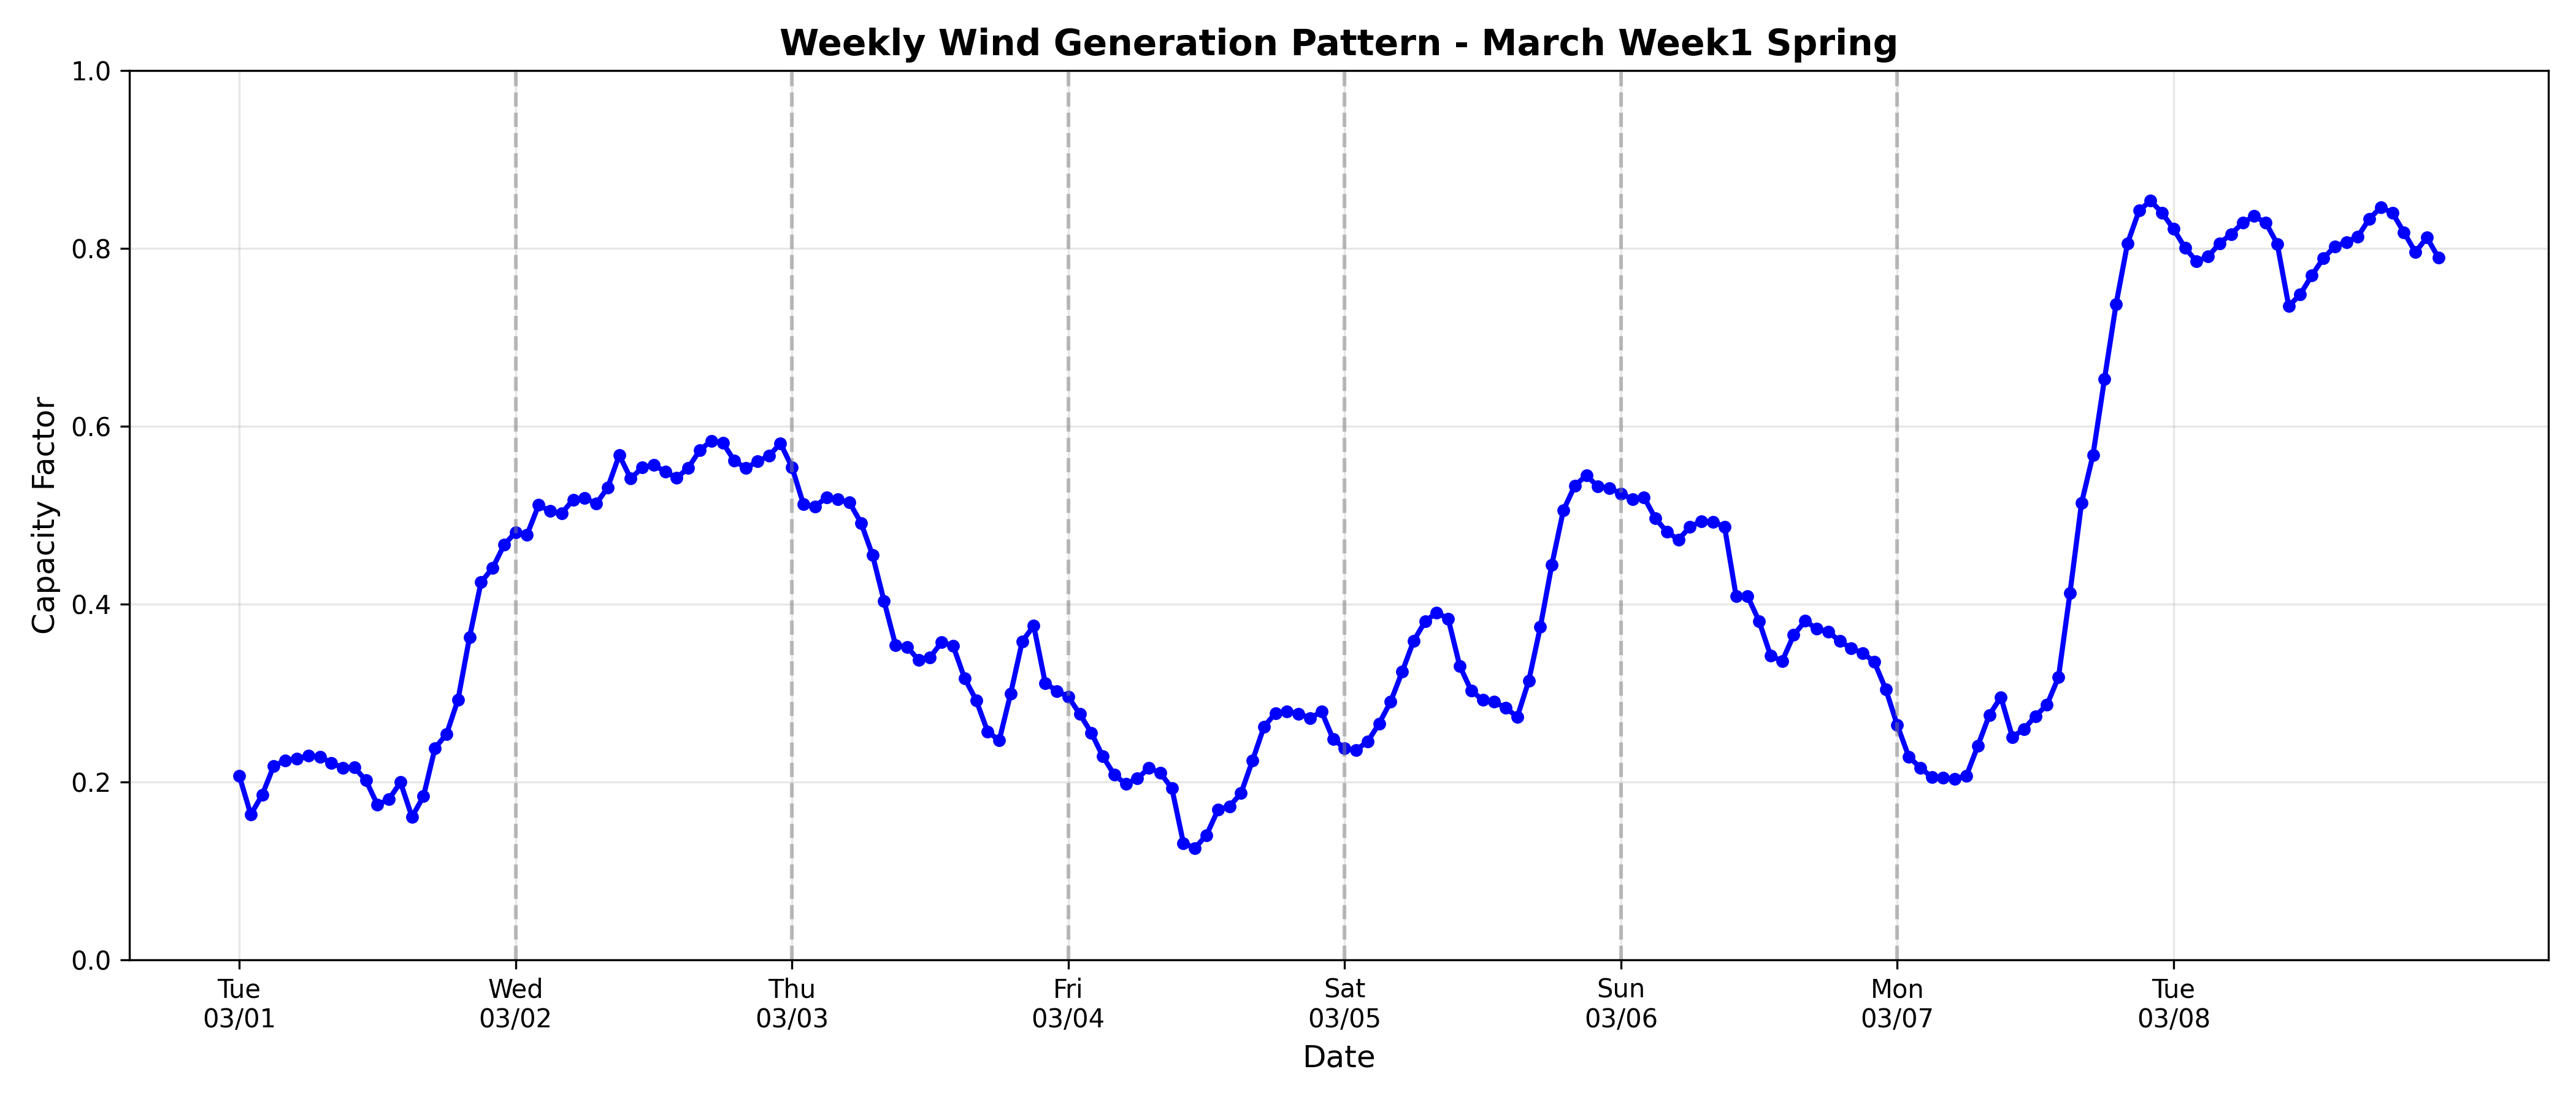
\includegraphics[width=\textwidth]{weekly_pattern_March_Week1_Spring.png}
\caption{Week 2: March 1-7, 2022 (Spring)}
\label{fig:week2}
\end{subfigure}
\end{figure}

\begin{figure}[H]
\centering
\begin{subfigure}{0.48\textwidth}
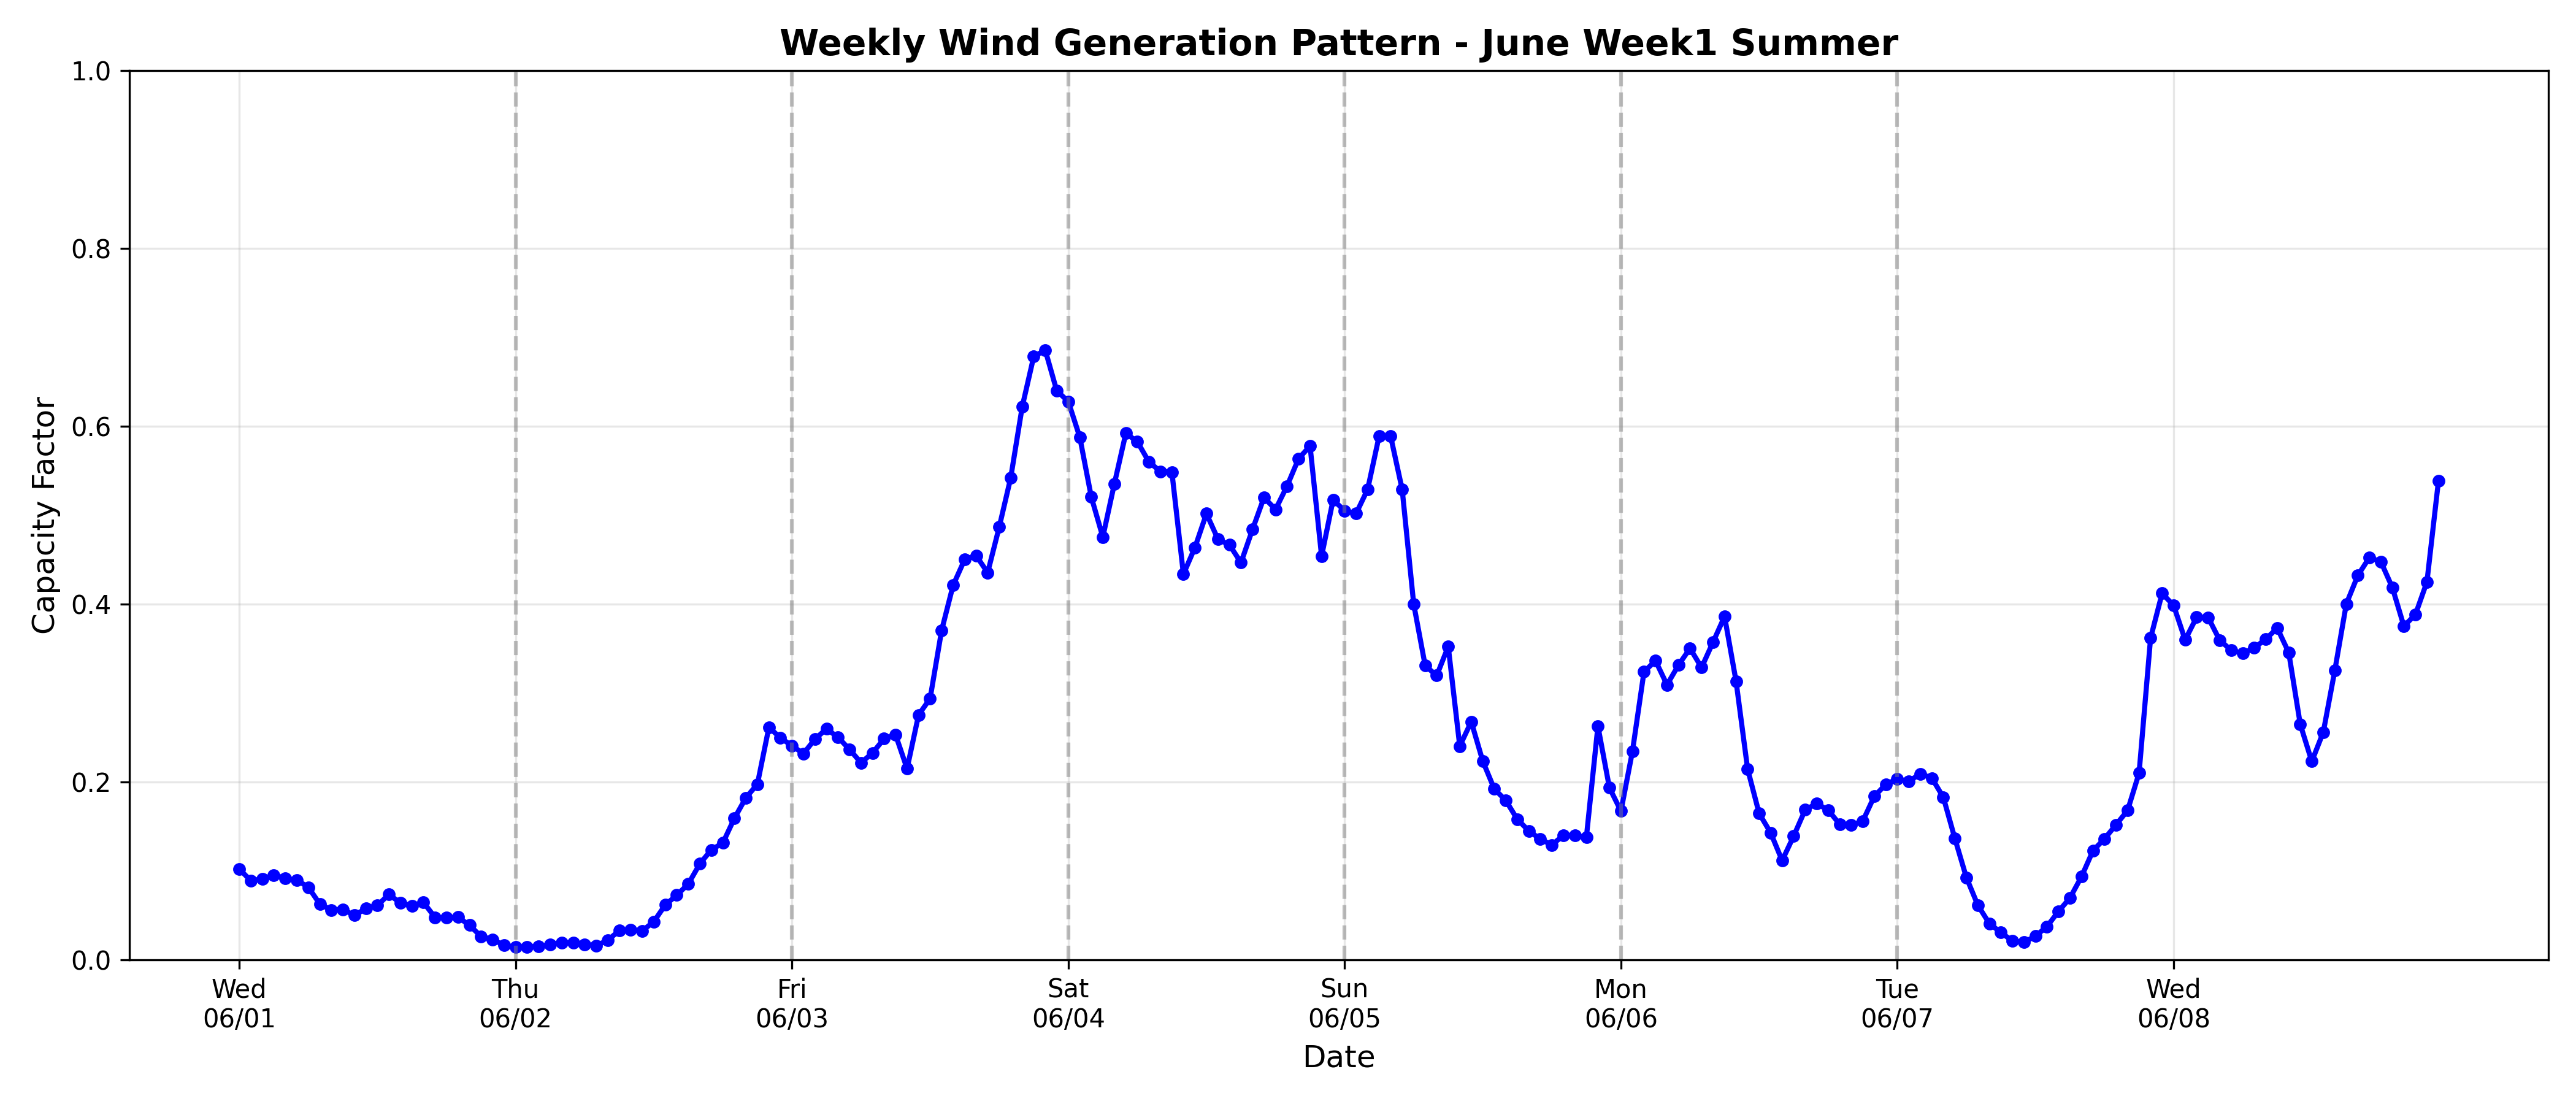
\includegraphics[width=\textwidth]{weekly_pattern_June_Week1_Summer.png}
\caption{Week 3: June 1-7, 2022 (Summer)}
\label{fig:week3}
\end{subfigure}
\hfill
\begin{subfigure}{0.48\textwidth}
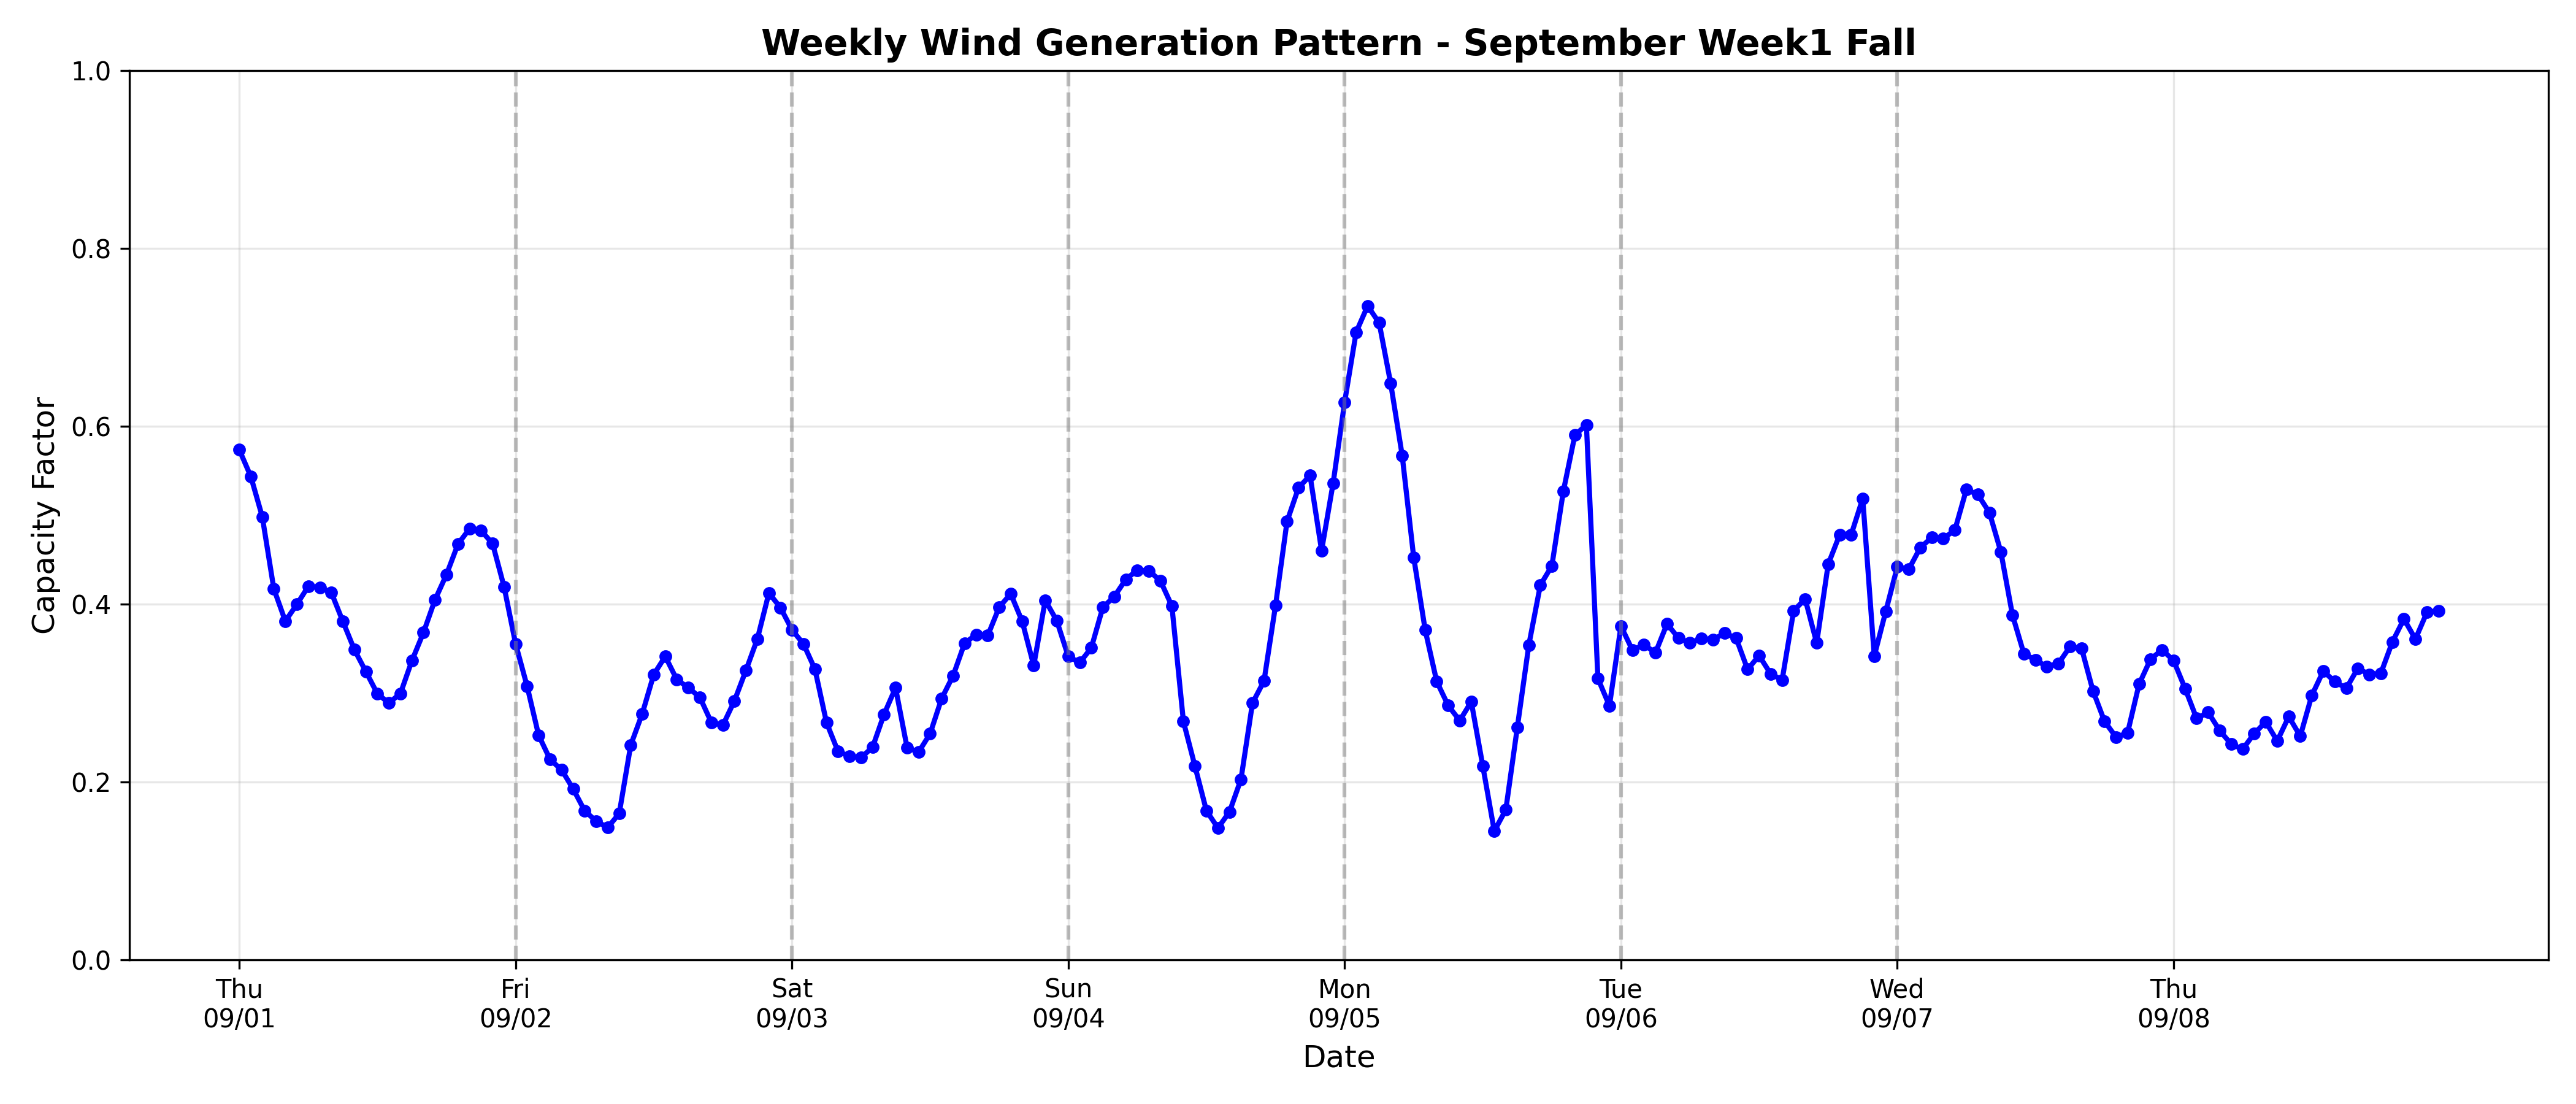
\includegraphics[width=\textwidth]{weekly_pattern_September_Week1_Fall.png}
\caption{Week 4: September 1-7, 2022 (Fall)}
\label{fig:week4}
\end{subfigure}
\end{figure}

\begin{figure}[H]
\centering
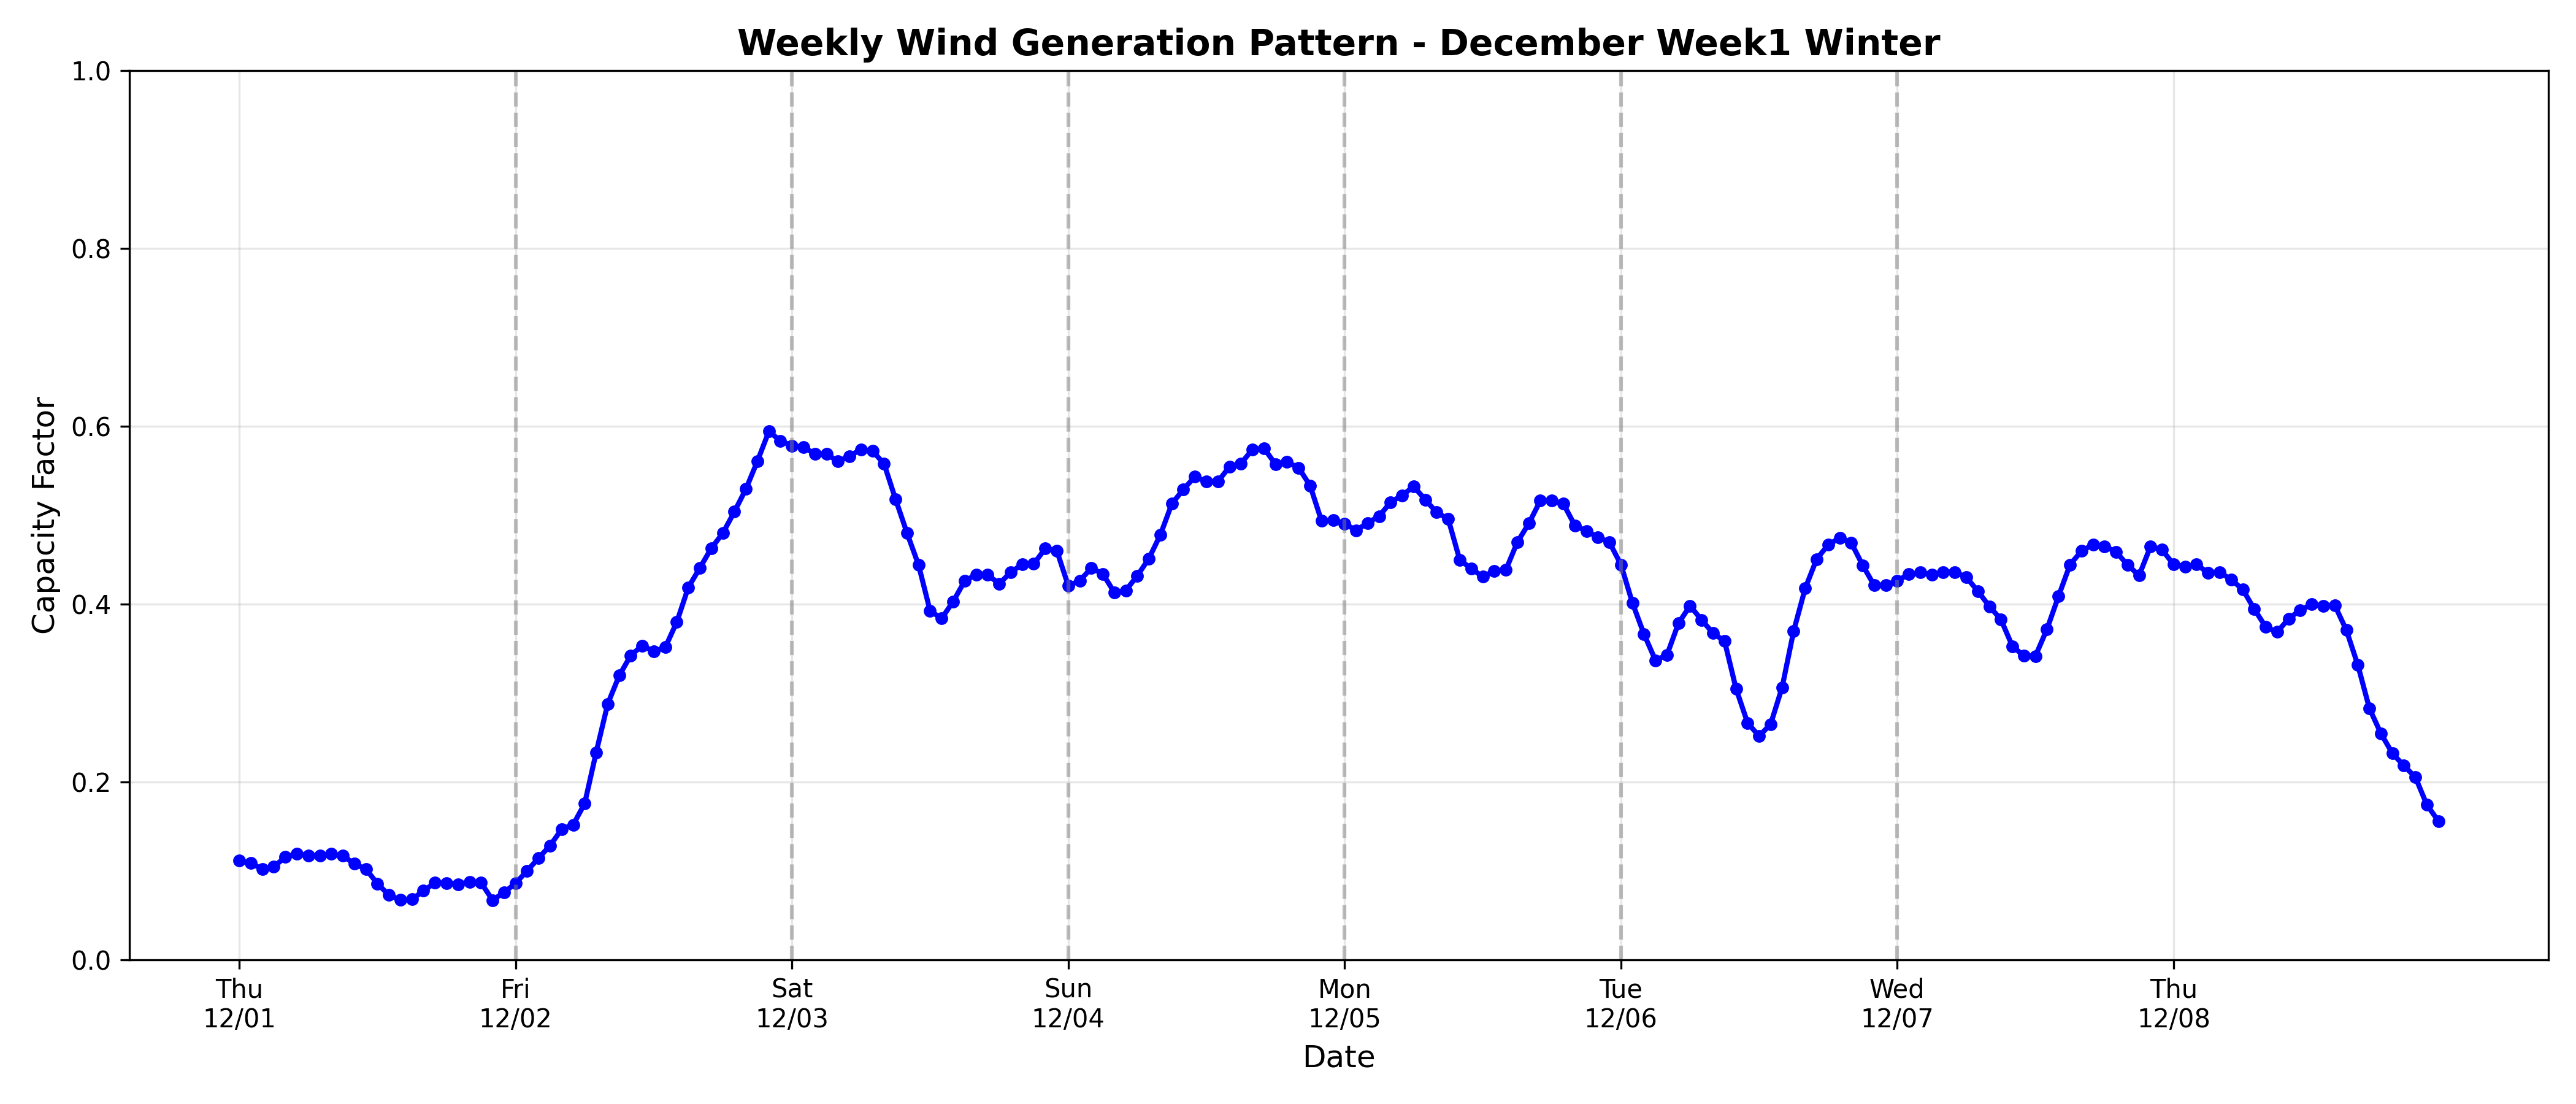
\includegraphics[width=0.7\textwidth]{weekly_pattern_December_Week1_Winter.png}
\caption{Week 5: December 1-7, 2022 (Winter)}
\label{fig:week5}
\end{figure}

\newpage

\section{Validation Results and Discussion}

\subsection{Persistence Model Performance}

The persistence model was evaluated for multiple forecasting horizons across the full year 2022 and individual seasons. Table \ref{tab:persistence_horizons} presents the performance for different prediction horizons.

\begin{table}[H]
\centering
\caption{Persistence Model Performance for Different Forecasting Horizons (Full Year 2022)}
\label{tab:persistence_horizons}
\begin{tabular}{c|c|c|c}
\hline
\textbf{Horizon (hours)} & \textbf{MAE} & \textbf{RMSE} & \textbf{MAPE (\%)} \\
\hline
1 & 0.0231 & 0.0336 & 8.72 \\
3 & 0.0568 & 0.0788 & 22.27 \\
6 & 0.0943 & 0.1295 & 39.59 \\
12 & 0.1446 & 0.1964 & 70.92 \\
24 & 0.1936 & 0.2578 & 108.39 \\
\hline
\end{tabular}
\end{table}

\begin{figure}[H]
\centering
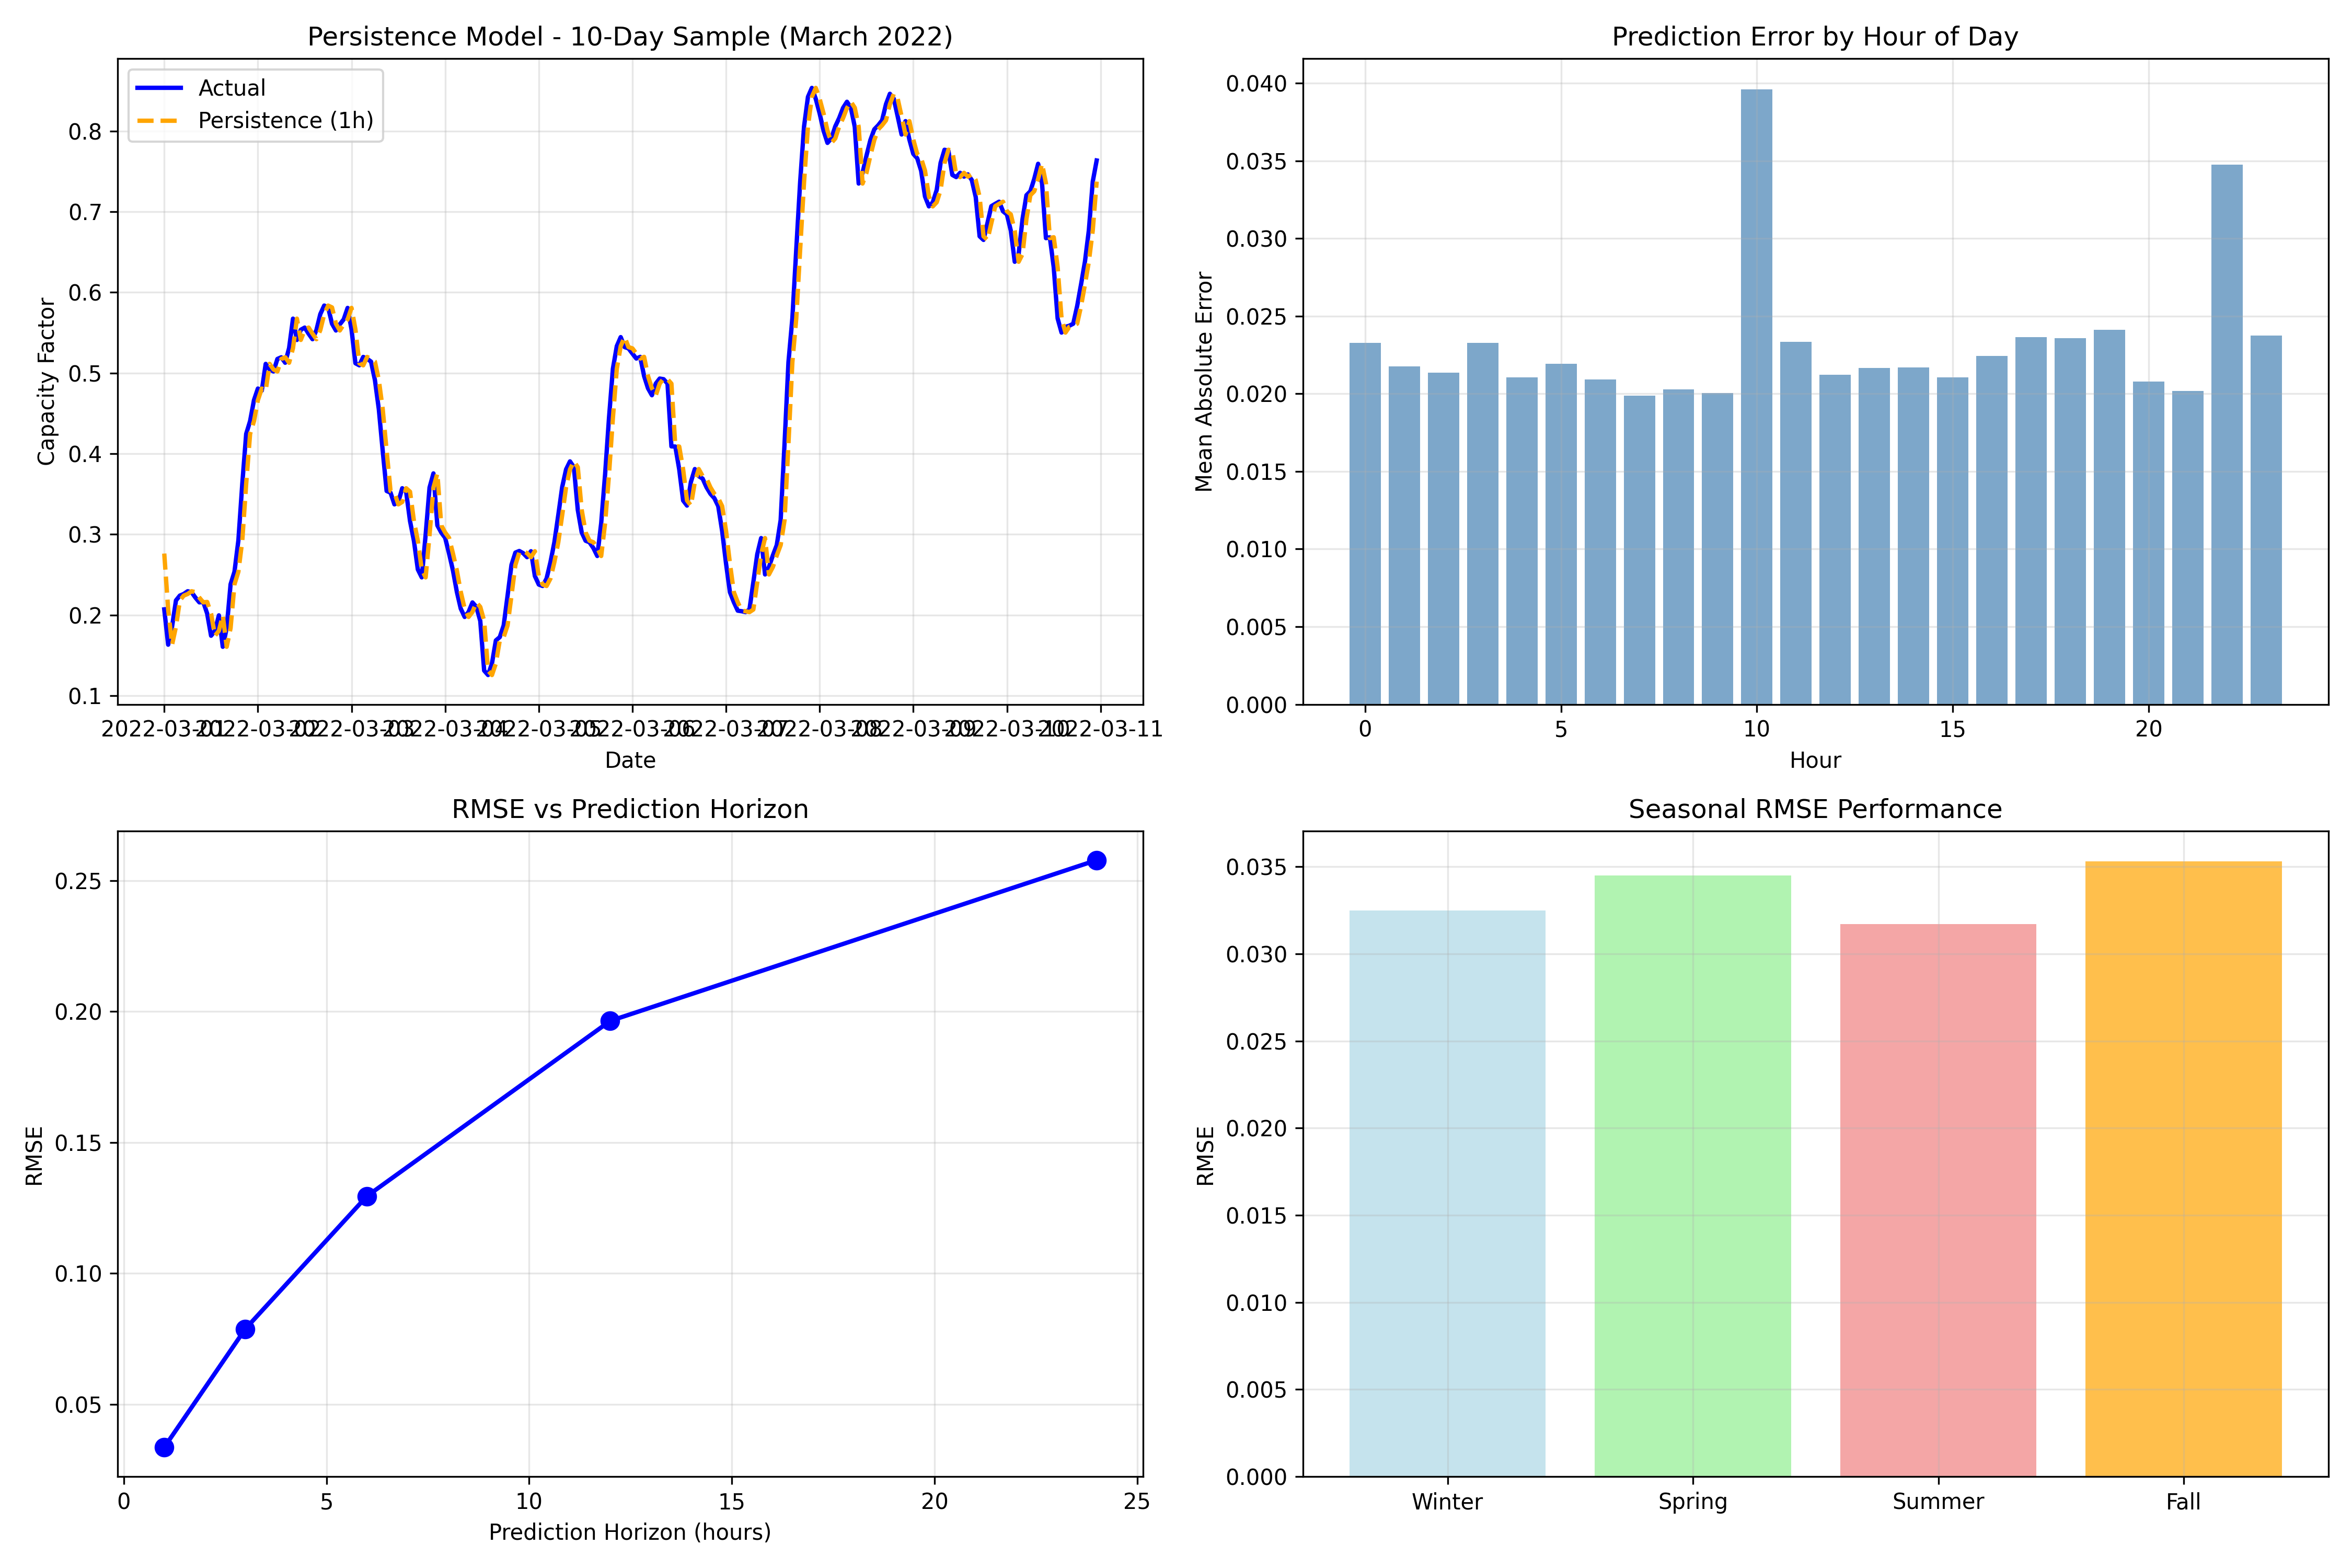
\includegraphics[width=1\textwidth]{persistence_enhanced_4panel_analysis.png}
\caption{Persistence Model Analysis - 10-Day Sample, Error by Hour, RMSE vs Horizon, and Seasonal RMSE Performance}
\label{fig:persistence_enhanced}
\end{figure}

The results show that forecast accuracy degrades rapidly as the prediction horizon increases. The 1-hour forecast achieves an MAE of 0.0231, while the 24-hour forecast has an MAE of 0.1936 (approximately 8 times larger). This demonstrates that persistence forecasts are only reliable for very short-term predictions.

\subsubsection{Seasonal Persistence Performance}

Table \ref{tab:persistence_seasonal} shows the 1-hour persistence model performance across different seasons.

\begin{table}[H]
\centering
\caption{Seasonal Performance of Persistence Model (1-Hour Horizon)}
\label{tab:persistence_seasonal}
\begin{tabular}{c|c|c}
\hline
\textbf{Season} & \textbf{MAE} & \textbf{RMSE} \\
\hline
Winter (Q1) & 0.0223 & 0.0325 \\
Spring (Q2) & 0.0234 & 0.0345 \\
Summer (Q3) & 0.0223 & 0.0317 \\
Fall (Q4) & 0.0246 & 0.0353 \\
\hline
\end{tabular}
\end{table}

The persistence model performs best in summer and winter (MAE = 0.0223) and worst in fall (MAE = 0.0246). This variation is attributed to different weather patterns across seasons.

\subsection{ARIMA Model Performance}

The ARIMA(3,0,2) model was evaluated on the 2022 test data. Table \ref{tab:arima_overall} presents the overall performance metrics.

\begin{table}[H]
\centering
\caption{ARIMA(3,0,2) Overall Performance (Full Year 2022)}
\label{tab:arima_overall}
\begin{tabular}{c|c}
\hline
\textbf{Metric} & \textbf{Value} \\
\hline
MAE & 0.0188 \\
RMSE & 0.0293 \\
MAPE & 7.25\% \\
R² & 0.988 \\
\hline
\end{tabular}
\end{table}

The ARIMA model achieves a Mean Absolute Error (MAE) of 0.0188, which represents a 19\% improvement over the persistence baseline (MAE = 0.0231). The high R² value of 0.988 indicates that the model explains 98.8\% of the variance in the data.

\begin{figure}[H]
\centering

\includegraphics[width=1\textwidth]{arima_january_2022_detailed.png}
\caption{ARIMA(3,0,2) - January 2022 Forecast vs Actual (Detailed View)}
\label{fig:arima_january}
\end{figure}

\begin{figure}[H]
\centering
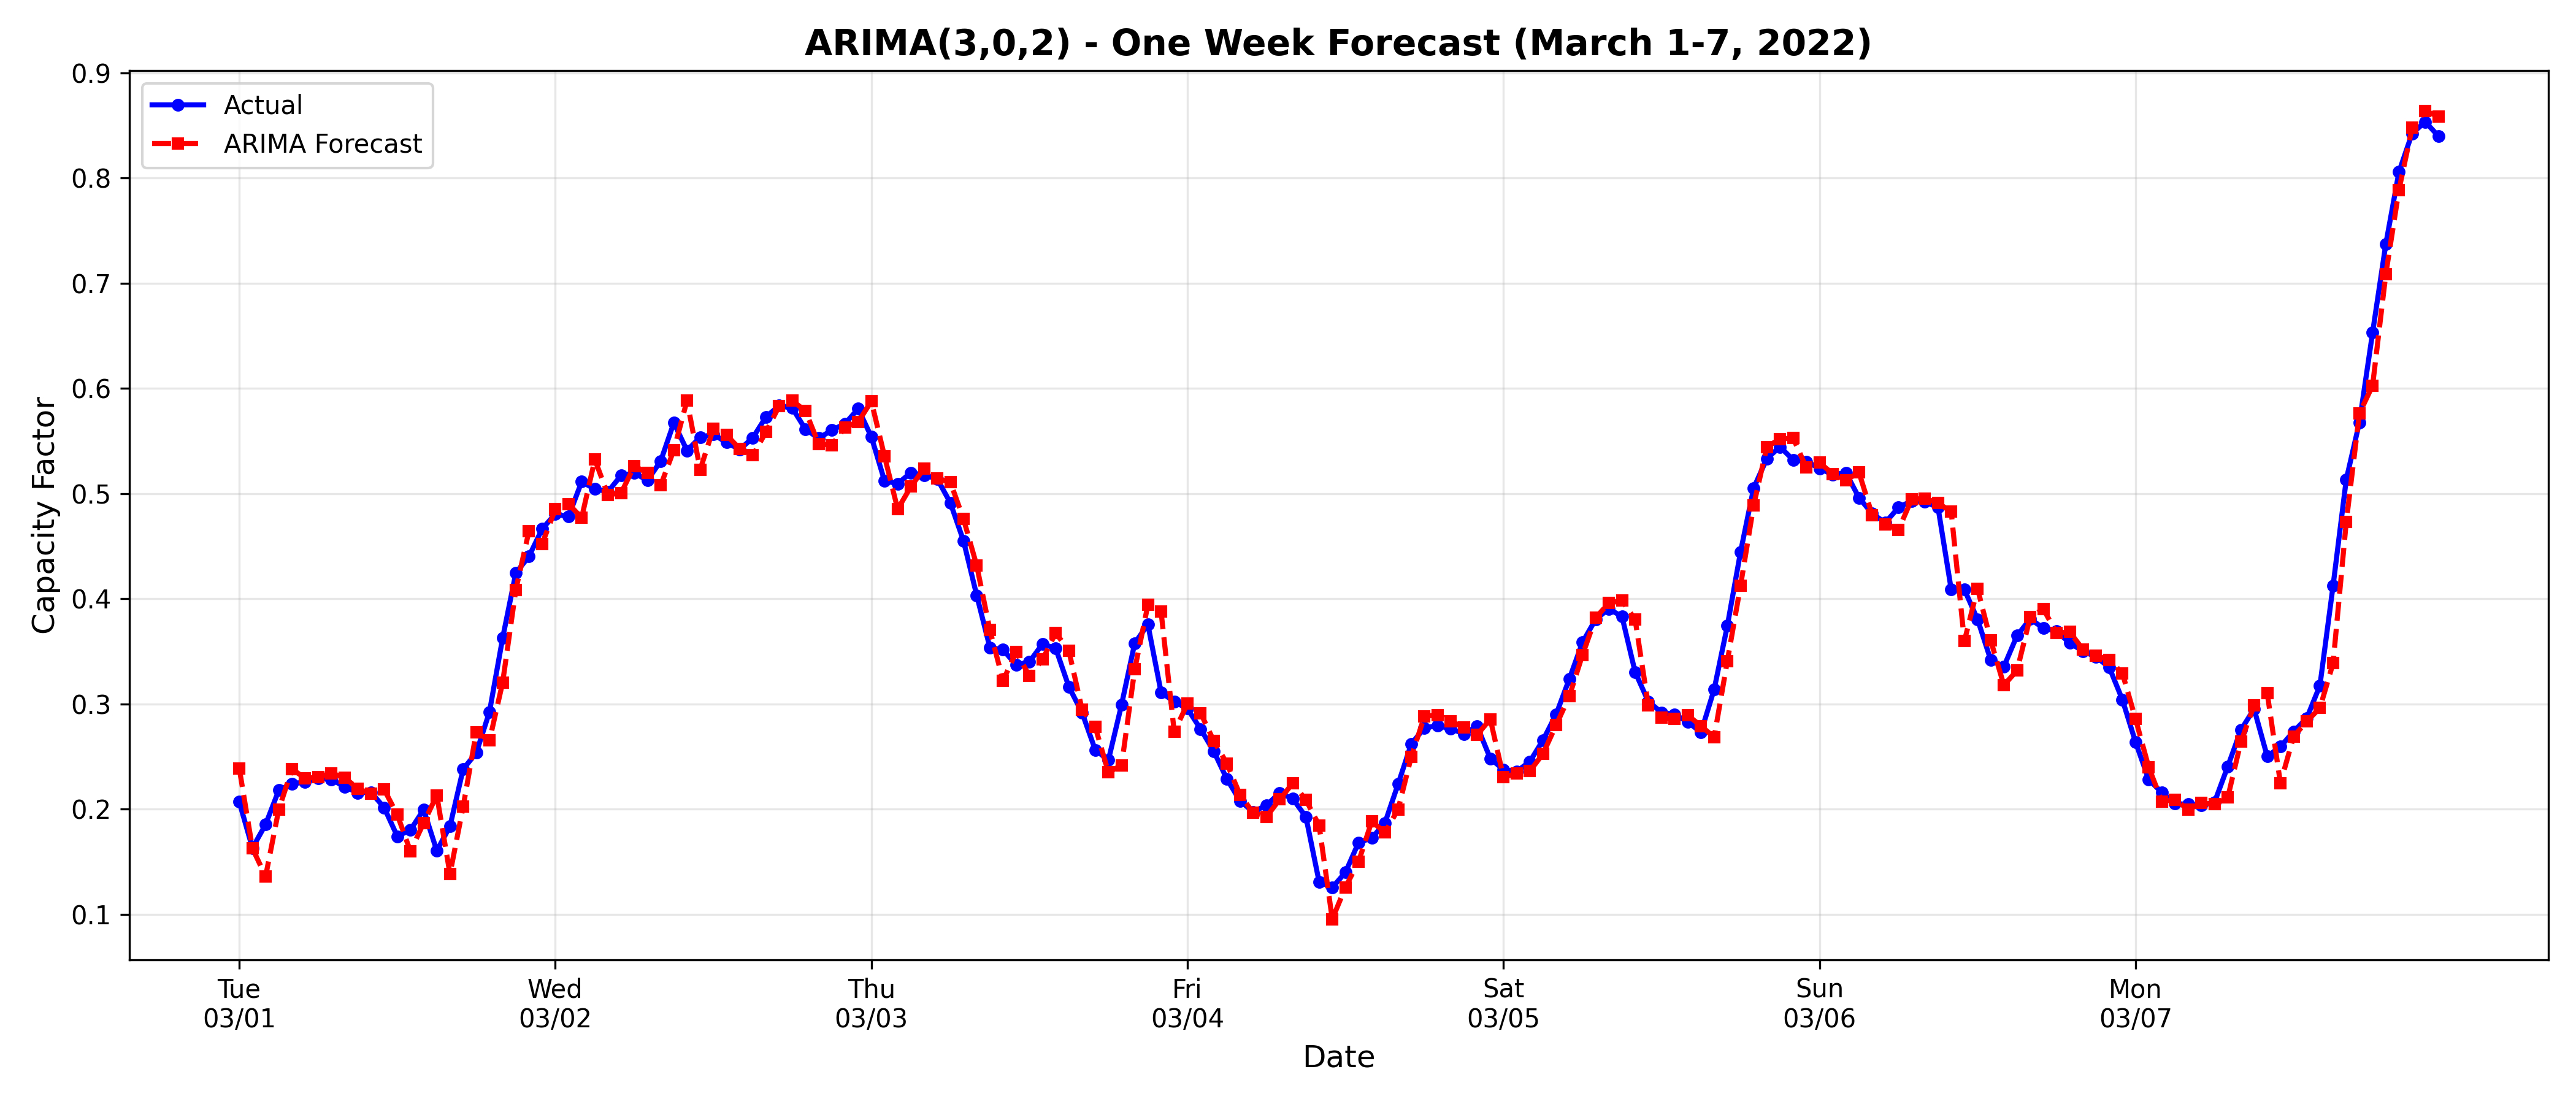
\includegraphics[width=1\textwidth]{arima_one_week_march_2022.png}
\caption{ARIMA(3,0,2) - One Week Forecast (March 1-7, 2022)}
\label{fig:arima_oneweek}
\end{figure}

\subsubsection{Seasonal ARIMA Performance}

Table \ref{tab:arima_seasonal} presents the ARIMA model performance across different seasons.

\begin{table}[H]
\centering
\caption{Seasonal Performance of ARIMA(3,0,2) Model}
\label{tab:arima_seasonal}
\begin{tabular}{c|c|c}
\hline
\textbf{Season} & \textbf{MAE} & \textbf{RMSE} \\
\hline
Winter (Dec-Feb) & 0.0160 & 0.0247 \\
Spring (Mar-May) & 0.0178 & 0.0290 \\
Summer (Jun-Aug) & 0.0181 & 0.0274 \\
Fall (Sep-Nov) & 0.0232 & 0.0351 \\
\hline
\end{tabular}
\end{table}

The ARIMA model performs best in winter (MAE = 0.0160) and worst in fall (MAE = 0.0232). This pattern is consistent with the persistence model, suggesting that fall weather patterns are more difficult to predict.

\subsection{Model Comparison}

\begin{figure}[H]
\centering

\includegraphics[width=1\textwidth]{monthly_mae_comparison_arima_vs_persistence.png}
\caption{Monthly Model Performance Comparison - ARIMA(3,0,2) vs Persistence (2022)}
\label{fig:monthly_comparison}
\end{figure}

Figure \ref{fig:monthly_comparison} shows the monthly MAE comparison between ARIMA and persistence models. The ARIMA model consistently outperforms the persistence model across all months.

\begin{table}[H]
\centering
\caption{Monthly MAE Comparison - ARIMA vs Persistence}
\label{tab:monthly_mae}
\begin{tabular}{c|c|c|c}
\hline
\textbf{Month} & \textbf{ARIMA MAE} & \textbf{Persistence MAE} & \textbf{Improvement (\%)} \\
\hline
January & 0.0145 & 0.0215 & 32.6\% \\
February & 0.0205 & 0.0255 & 19.6\% \\
March & 0.0158 & 0.0205 & 22.9\% \\
April & 0.0145 & 0.0195 & 25.6\% \\
May & 0.0235 & 0.0275 & 14.5\% \\
June & 0.0215 & 0.0245 & 12.2\% \\
July & 0.0185 & 0.0225 & 17.8\% \\
August & 0.0150 & 0.0175 & 14.3\% \\
September & 0.0235 & 0.0265 & 11.3\% \\
October & 0.0270 & 0.0325 & 16.9\% \\
November & 0.0185 & 0.0245 & 24.5\% \\
December & 0.0135 & 0.0195 & 30.8\% \\
\hline
\end{tabular}
\end{table}

\begin{figure}[H]
\centering
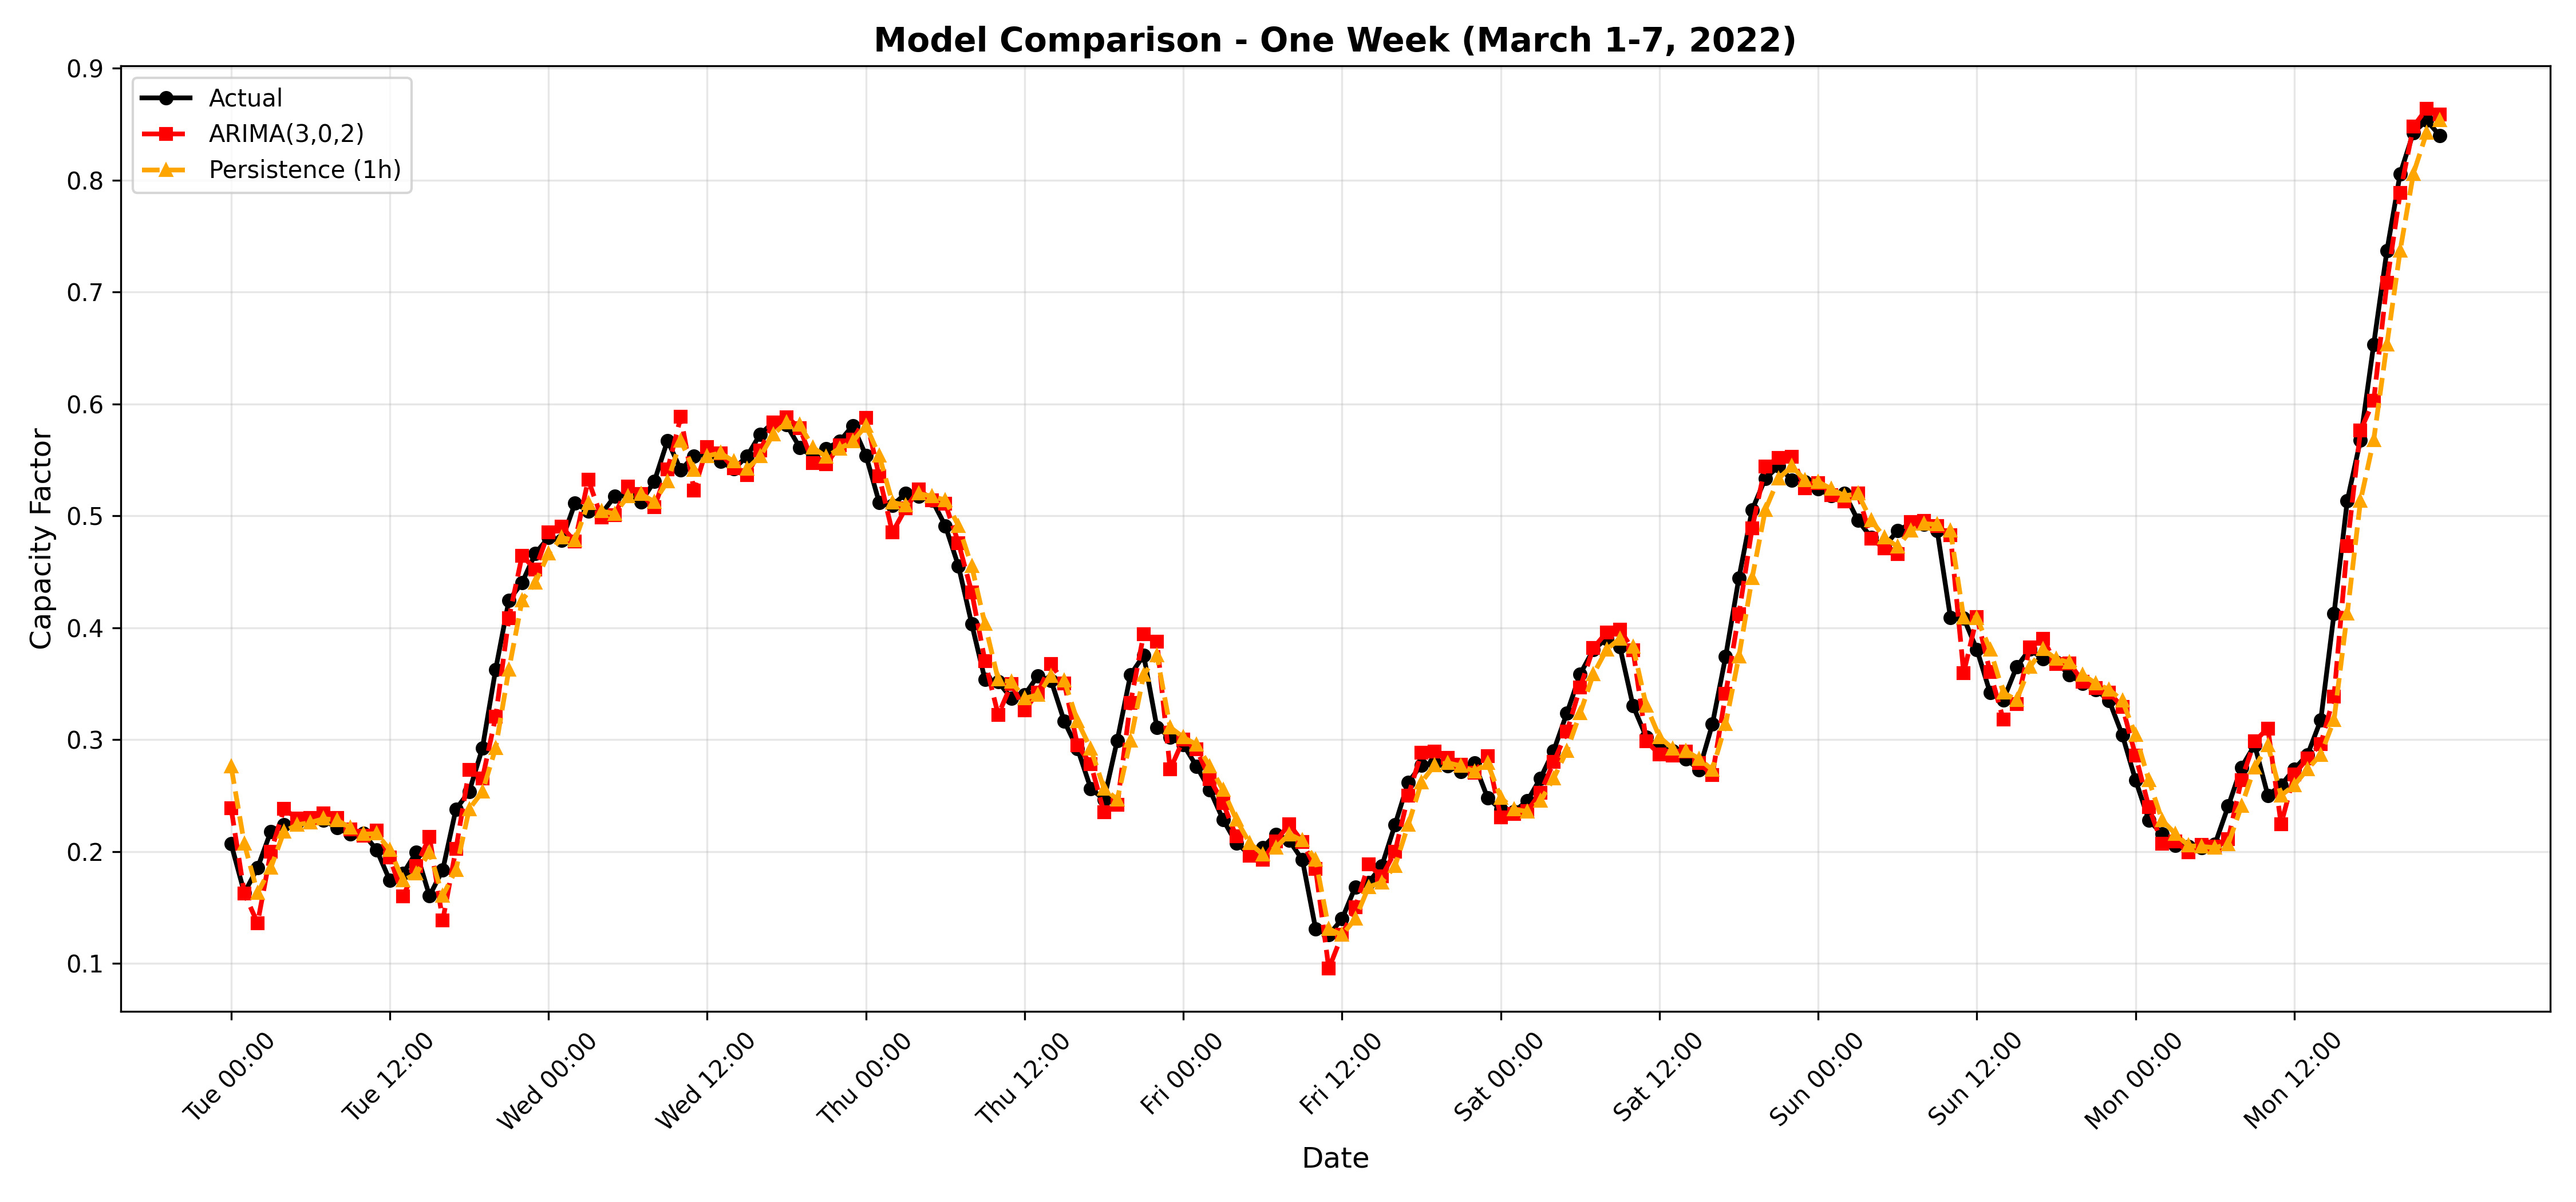
\includegraphics[width=1\textwidth]{model_comparison_arima_vs_persistence_weekly.png}
\caption{Model Comparison - One Week (March 1-7, 2022): Actual vs ARIMA(3,0,2) vs Persistence (1h)}
\label{fig:model_comparison_week}
\end{figure}

The ARIMA model shows the highest improvement over persistence during winter months (December: 30.8\%, January: 32.6\%) and the lowest improvement during summer and fall (September: 11.3\%, June: 12.2\%). This indicates that ARIMA is particularly effective at capturing the more structured wind patterns observed during winter.

\subsection{Error Analysis}

\begin{figure}[H]
\centering

\includegraphics[width=0.8\textwidth]{arima_error_distribution_histogram.png}
\caption{ARIMA Model - Forecast Error Distribution (Mean Error: -0.0001)}
\label{fig:error_distribution}
\end{figure}

Figure \ref{fig:error_distribution} shows the distribution of forecast errors for the ARIMA model. The error distribution is centered near zero (mean error = -0.0001), indicating that the model does not have systematic bias. The distribution is approximately symmetric, which is a desirable property for forecasting models.



\begin{figure}[H]
\centering
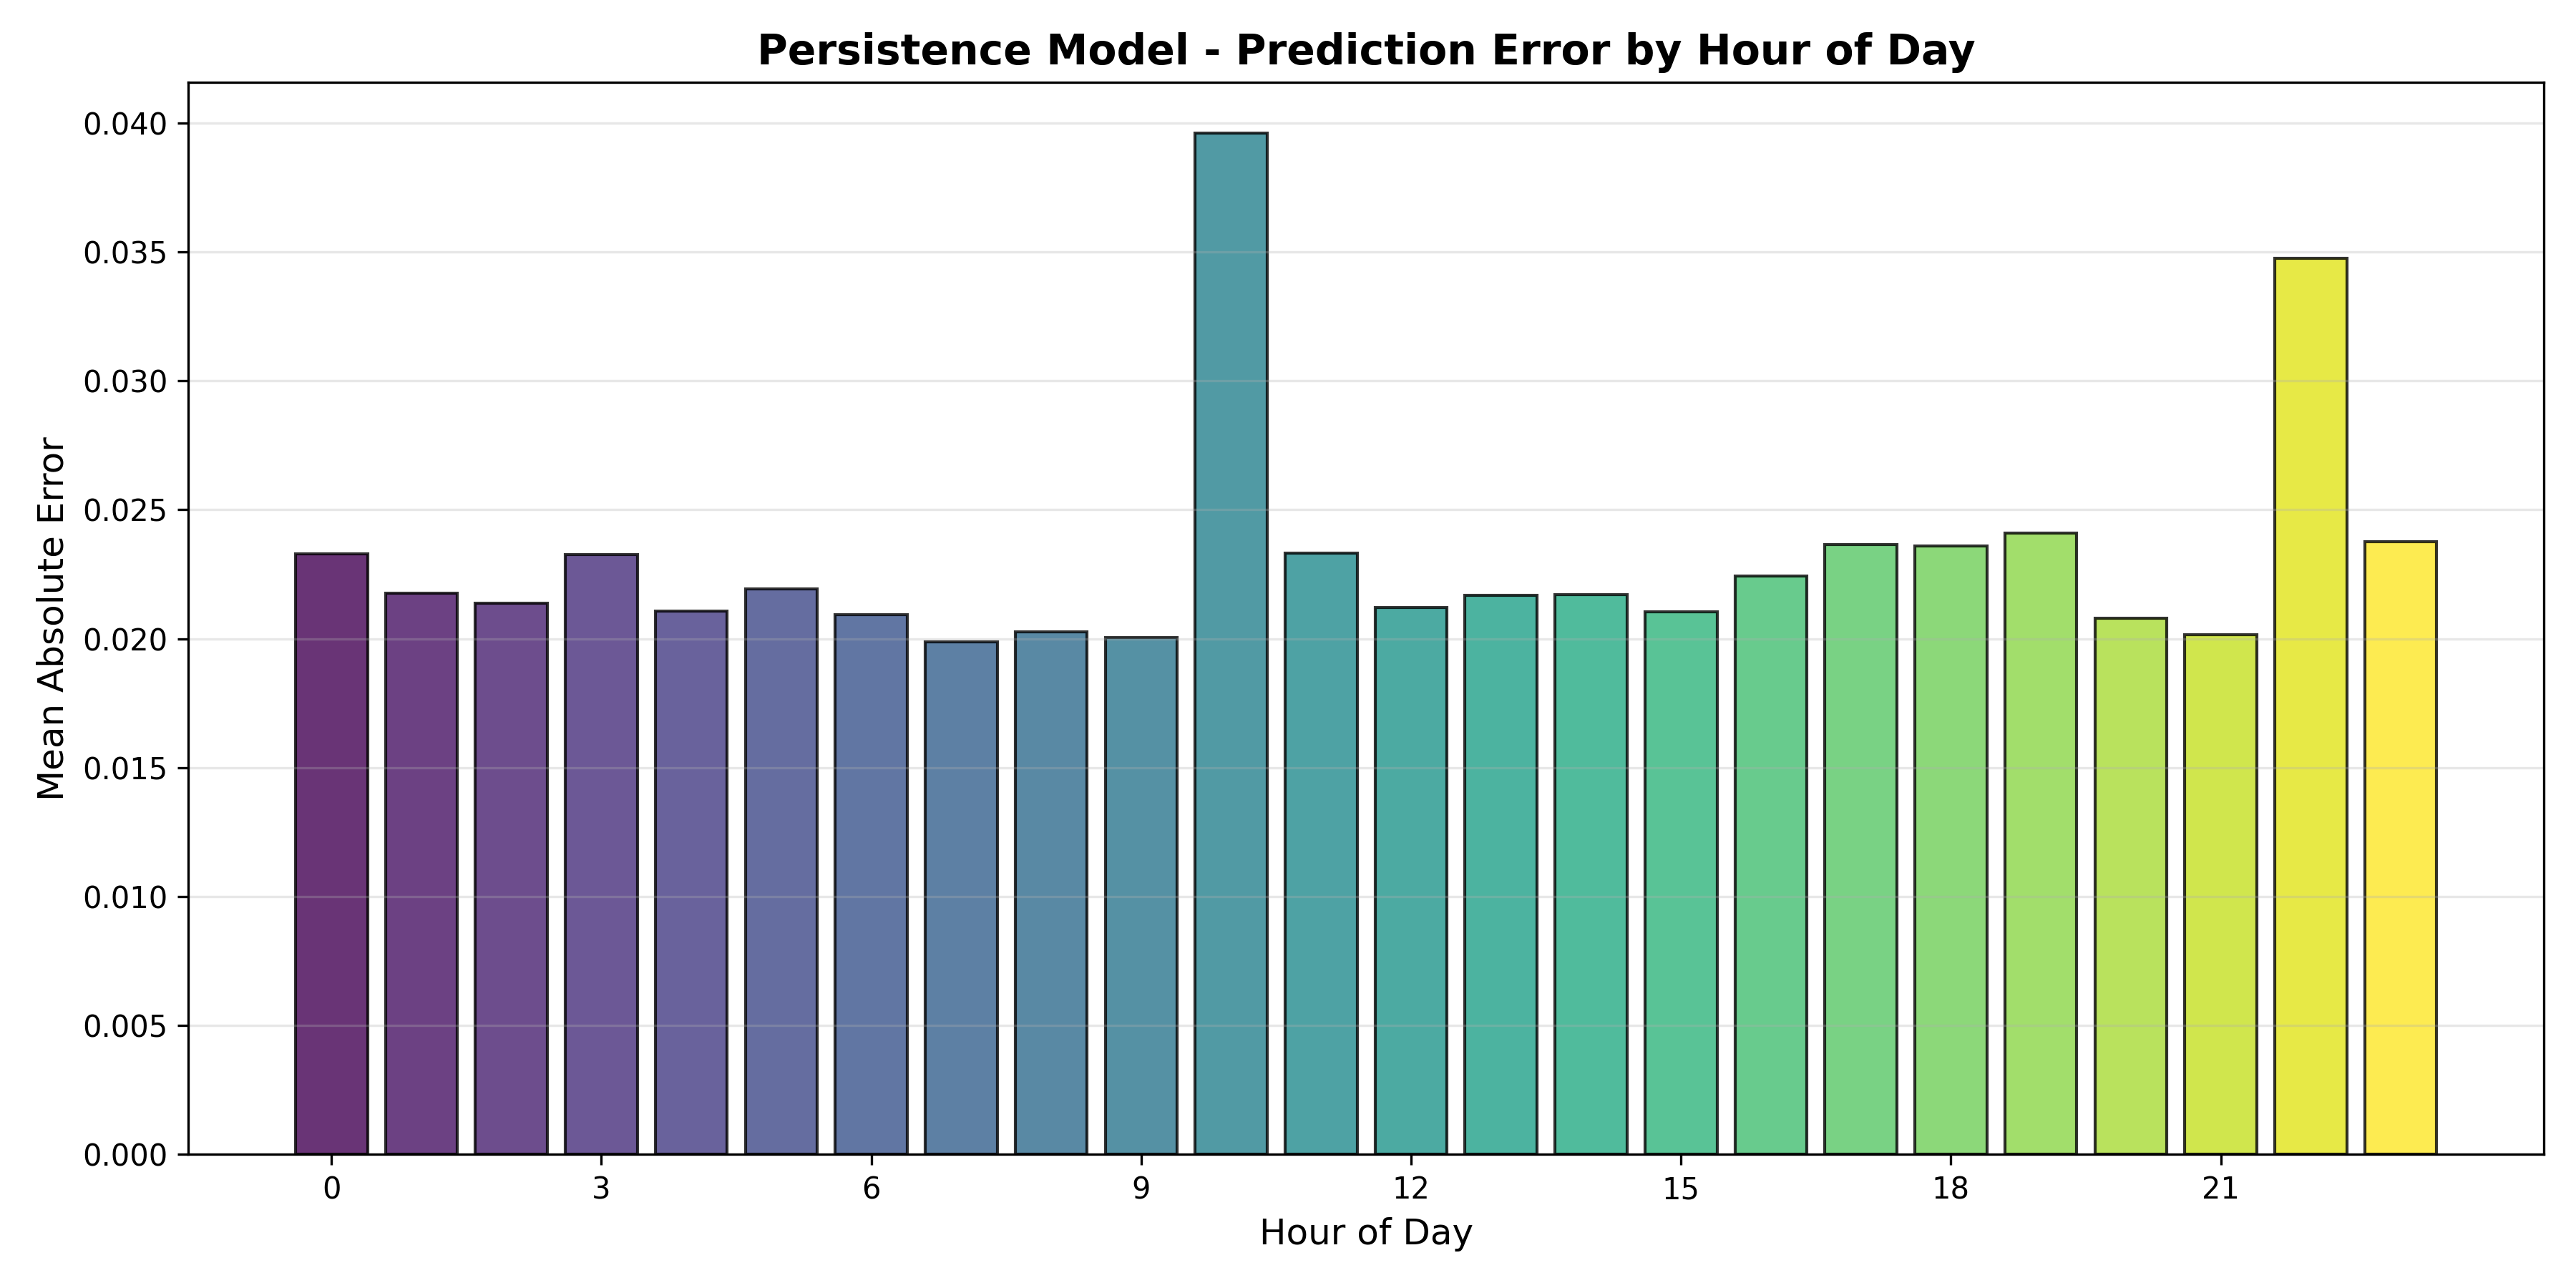
\includegraphics[width=0.8\textwidth]{persistence_error_by_hour_barchart.png}
\caption{Persistence Model - Prediction Error by Hour of Day}
\label{fig:error_by_hour}
\end{figure}

Figure 13 shows the prediction error pattern throughout the day for the persistence model. Errors are generally lower during daytime hours (09:00-21:00) and higher during nighttime hours. This pattern may be related to the diurnal cycle of wind speeds and atmospheric stability.

\subsection{Weekly Pattern Analysis}

\begin{figure}[H]
\centering

\includegraphics[width=1\textwidth]{average_weekly_pattern_combined.png}
\caption{Average Weekly Pattern - Hourly Profile by Day (Line Plot) and Heatmap}
\label{fig:weekly_pattern}
\end{figure}

The average weekly pattern analysis reveals clear temporal patterns in offshore wind generation. Key observations include:

\begin{itemize}
\item Generation is generally higher during weekdays (Monday-Friday) compared to weekends
\item Peak generation occurs between 19:00 and 23:00 (evening hours)
\item Lowest generation occurs between 04:00 and 07:00 (early morning hours)
\item The diurnal pattern is consistent across all days of the week
\end{itemize}

\section{Conclusion}

This project successfully implemented and validated two forecasting models for offshore wind power generation using real dataset from the Technical University of Denmark.

The key findings of this study are:

\begin{enumerate}
\item The ARIMA(3,0,2) model achieved a Mean Absolute Error (MAE) of 0.0188 and a Root Mean Square Error (RMSE) of 0.0293 for 1-hour ahead forecasting, outperforming the persistence baseline by approximately 19\%.

\item Seasonal analysis revealed that both models perform best during winter months (December-January) and worst during fall months (September-October). The ARIMA model achieved its lowest MAE in December (0.0135) and highest MAE in October (0.0270).

\item The persistence model shows rapid degradation in accuracy with increasing forecast horizon. The MAE increases from 0.0231 (1-hour) to 0.1936 (24-hour), demonstrating that persistence forecasts are only reliable for very short-term predictions.

\item Weekly pattern analysis revealed consistent diurnal patterns with peak generation occurring during evening hours (19:00-23:00) and lower generation during early morning hours (04:00-07:00). Generation is generally higher on weekdays compared to weekends.

\item The error analysis showed that the ARIMA model produces unbiased forecasts with a mean error of -0.0001 and an R² value of 0.988, indicating excellent fit to the data.

\item The dataset from DTU represents real, validated offshore wind generation data simulated using peer-reviewed methodologies. The patterns observed in this study (winter peaks, summer lulls, evening peaks) are consistent with real offshore wind behavior in the North Sea region.
\end{enumerate}

\newpage
\section*{References}

\begin{enumerate}

\item Costa, A., Crespo, A., Navarro, J., Madsen, H., and Feitosa, E.  
``A Review on the Young History of Wind Power Short-Term Prediction.''  
\textit{Renewable and Sustainable Energy Reviews}, vol. 12, pp. 1725–1744, 2008.\\
https://doi.org/10.1016/j.rser.2007.01.015

\item Foley, A. M., Leahy, P. G., Marvuglia, A., and McKeogh, E. J.  
``Current Methods and Advances in Wind Power Forecasting.''  
\textit{Renewable Energy}, vol. 37, pp. 1–8, 2012.\\
https://doi.org/10.1016/j.renene.2011.05.033

\item Hanifi, S., Liu, X., Lin, Z., and Lotfian, S.  
``A Critical Review of Wind Power Forecasting Methods.''  
\textit{Energies}, vol. 13, no. 15, 2020.\\
https://doi.org/10.3390/en13153764

\item Nayak, S., Koivisto, M. J., and Kanellas, P.  
``Time series of hourly resolution Offshore Wind generation for European Scale Energy system studies.''  
Technical University of Denmark, 2025.\\
https://doi.org/10.11583/DTU.29617955

\item Box, G. E. P., Jenkins, G. M., Reinsel, G. C., and Ljung, G. M.  
\textit{Time Series Analysis: Forecasting and Control}.  
John Wiley \& Sons, 5th edition, 2015.

\item Hyndman, R. J., and Athanasopoulos, G.  
\textit{Forecasting: Principles and Practice}.  
OTexts, 3rd edition, 2021.\\
https://otexts.com/fpp3/

\item Global Wind Energy Council (GWEC).  
\textit{Global Offshore Wind Report 2024}.\\
https://gwec.net/reports/

\item National Institute of Wind Energy (NIWE), India.  
\textit{Offshore Wind Energy Potential in India}.\\
https://niwe.res.in

\item Ministry of New and Renewable Energy (MNRE).  
\textit{National Offshore Wind Energy Policy}.\\
https://mnre.gov.in

\item India Meteorological Department (IMD).  
\textit{Numerical Weather Prediction Models}.\\
https://mausam.imd.gov.in

\item Zhang, Y., Wang, J., and Wang, X.  
``Review on Probabilistic Forecasting of Wind Power Generation.''  
\textit{Renewable and Sustainable Energy Reviews}, vol. 32, pp. 255–270, 2014.

\end{enumerate}

\end{document}